\documentclass[12pt]{article}

% Times New Roman
\usepackage{newtxtext,newtxmath}

% Page formatting
\usepackage[a4paper,margin=1in]{geometry}
\usepackage{graphicx}
\usepackage{array}
\usepackage{setspace}
\usepackage{booktabs}
\usepackage{multirow}
\usepackage{tcolorbox}
\usepackage{algorithm}
\usepackage{algpseudocode}
\usepackage{natbib}
\usepackage{float}
\usepackage{hyperref}
\usepackage{tikz}
\usetikzlibrary{shapes,arrows,positioning,calc}

% Set bibliography style
\bibliographystyle{apalike}

\begin{document}

% ---------------- COVER PAGE ----------------
\begin{titlepage}
    \centering

    \vspace*{1.0cm}
    
    % UM LOGO (Make sure um-logo.png is in your folder)
    \includegraphics[width=10cm]{um-logo.png}\\[1.5cm]  

    % COURSE CODE + TITLE
    {\Large \textbf{WIB3003: Academic Project II}}\\[2cm]

    % PROJECT TITLE
    {\Large \textbf{Embedding-Based Suspicious Activity Recognition in Multi-Camera Video Feeds Using Lightweight Transformers}}\\[2cm]

    \renewcommand{\arraystretch}{1.5}
    \begin{tabular}{|l|l|}
        \hline
        \textbf{Name} & Badr Faez Salem Ba Jamil \\ \hline
        \textbf{Matric No.} & 22115571 \\ \hline
        \textbf{Supervisor} & Liew Wei Shiung \\ \hline
        \textbf{Semester/Session} & Semester 2, 2025/2026 \\ \hline
    \end{tabular}

    \vfill
    {\large Faculty of Computer Science \& Information Technology\\ University of Malaya}
    \vspace*{1cm}

\end{titlepage}

\clearpage

% ---------------- ABSTRACT ----------------
\begin{center}
    {\Large \textbf{Abstract}}\\[0.5cm]
\end{center}

\noindent The rapid expansion of surveillance networks necessitates automated systems capable of robust anomaly detection; however, existing methods often fail to balance computational efficiency with the detailed context required to distinguish complex behaviors. The objective of this project is to develop a real-time, hybrid system titled ``Embedding-Based Suspicious Activity Recognition in Multi-Camera Video Feeds Using Lightweight Transformers.'' 

\vspace{0.3cm}
\noindent The methodology implements a multi-stream fusion approach to decouple motion from appearance. YOLO11s-pose extracts a 96-dimensional skeletal representation, Lucas-Kanade optical flow produces a 64-dimensional polyline motion representation, and X3D-XS extracts a 192-dimensional visual feature vector. These streams are integrated via a Lightweight Transformer Fusion Module employing cross-attention, followed by a Deep Streaming Linear Discriminant Analysis (SLDA) classifier for real-time binary anomaly detection. Findings and discussion reveal that the proposed system achieves a video-level AUC-ROC of 0.9059 and frame-level AUC-ROC of 0.7554 on the UCF-Crime dataset. It effectively detects behaviors such as fighting, loitering, and falling while processing three concurrent video streams at $>$15 FPS on a consumer-grade NVIDIA RTX 3060. The practical implications of this research offer a privacy-preserving, edge-deployable security solution that significantly reduces hardware and cost barriers for intelligent surveillance. In conclusion, the system successfully bridges the gap between high-accuracy academic algorithms and resource-constrained real-world deployment, fulfilling all project objectives.

\vfill
\clearpage

% ---------------- TABLE OF CONTENTS ----------------
\tableofcontents
\clearpage

% ---------------- CHAPTER 1: INTRODUCTION ----------------
\section{Introduction}

\subsection{Project Overview}
As the domain of video surveillance evolves into the Internet of Video Things (IoVT), the research focus is shifting from purely algorithmic accuracy to the development of deployable \textbf{Networking Systems for Video Anomaly Detection (NSVAD)}. While deep learning has revolutionized anomaly detection, existing academic solutions often neglect the constraints of the \textit{Hardware} and \textit{System} layers, resulting in models that are computationally too expensive for real-time, multi-stream deployment on edge devices.

This project, titled \textbf{``Embedding-Based Suspicious Activity Recognition in Multi-Camera Video Feeds Using Lightweight Transformers,''} addresses these systemic gaps by developing a lightweight, privacy-aware AI system. Moving beyond heavy 3D-CNNs, this project implements a \textbf{multimodal fusion strategy} that decouples motion from appearance. The system utilizes \textbf{YOLO11s-pose} for rapid skeletal pose estimation—ensuring geometric precision and privacy—and \textbf{X3D-XS} for efficient visual context extraction. These streams are integrated via a \textbf{Lightweight Temporal Transformer} and classified using \textbf{Deep Streaming Linear Discriminant Analysis (SLDA)} \citep{hayes2020lifelong}. This architecture is specifically designed to process at least three concurrent video feeds on a single consumer-grade GPU with low latency, bridging the gap between high-performance AI and practical security deployment.

\subsection{Problem Statement}
According to the systematic review of Networking Systems for Video Anomaly Detection (NSVAD) by \cite{liu2024networking}, the deployment of effective anomaly detection in real-world scenarios is hindered by three critical limitations:

\begin{enumerate}
    \item \textbf{The Hardware-Algorithm Efficiency Gap:} \cite{liu2024networking} highlights a disconnect between the \textit{Algorithm Layer} and the \textit{Hardware Layer}. Current state-of-the-art models (e.g., I3D, ViT) prioritize accuracy over resource optimization, creating high computational overhead that prevents multi-stream processing on resource-constrained edge devices.
    
    \item \textbf{Privacy Leakage and Appearance Bias:} Traditional pixel-based approaches suffer from privacy concerns (P2VAD) as they process raw identifiable information. Furthermore, relying solely on RGB data introduces ``appearance bias,'' where models may incorrectly flag individuals based on clothing or background rather than behavioral anomalies.
    
    \item \textbf{Catastrophic Forgetting and Lack of Adaptability:} Traditional classification models lack the capacity for streaming or incremental learning. When deployed in dynamic environments, they suffer from catastrophic forgetting and cannot adapt to new camera viewpoints, environmental changes, or novel suspicious activity prototypes without undergoing full, computationally expensive retraining.
\end{enumerate}

\subsection{Project Objectives}
The primary objectives of this project are:
\begin{enumerate}
    \item Develop a multi-stream feature extraction pipeline utilizing YOLO11s-pose (Skeletal) and X3D-XS (Appearance).
    \item Design a Lightweight Temporal Transformer to fuse multimodal data and capture long-range temporal dependencies.
    \item Implement a Deep Streaming Linear Discriminant Analysis (SLDA) classifier for prototype-based anomaly detection.
    \item Evaluate the system on the UCF-Crime dataset, targeting $>$15 FPS processing speed and $<$2 seconds latency on consumer hardware.
\end{enumerate}

\subsection{Project Scope}
\begin{itemize}
    \item \textbf{Dataset:} UCF-Crime and NTU RGB+D (Focus: Fighting, Loitering, Abuse).
    \item \textbf{Hardware:} Optimized for NVIDIA RTX 3060 (Consumer-grade).
    \item \textbf{Input:} Minimum of three concurrent video streams.
    \item \textbf{Technique:} Weakly Supervised Learning and Prototype-based classification.
\end{itemize}

\subsection{Project Significance}
This research bridges the gap between academic algorithms and deployable security solutions. By utilizing SLDA and lightweight transformers, it offers a privacy-preserving, scalable solution that reduces false positives and adapts to new threats without requiring full model retraining.

\clearpage


% ---------------- CHAPTER 2: LITERATURE REVIEW ----------------
\section{Literature Review}

\subsection{Introduction}
The domain of Video Anomaly Detection (VAD) has evolved significantly from manual feature engineering to sophisticated deep learning approaches. With the expansion of the Internet of Video Things (IoVT), recent trends emphasize Privacy-Preserving VAD (P2VAD) and Networking Systems for Video Anomaly Detection (NSVAD), focusing on practical deployability, resource efficiency, real-time processing, and ethical considerations in real-world surveillance applications \citep{liu2024networking, liu2025privacy}. VAD aims to automatically identify unexpected spatial-temporal patterns in video sequences that deviate from normal behavior, enabling intelligent systems to flag security threats, traffic accidents, and other critical events without continuous human monitoring. This chapter reviews the primary VAD research paradigms, illustrated in Figure \ref{fig:vad_frameworks}, and positions the proposed system within this landscape.

% --- FIGURE INSERTION ---
\begin{figure}[htbp]
    \centering
    \includegraphics[width=1.0\textwidth]{vad_frameworks.png} 
    \caption{Comparison of learning frameworks: (a) Unsupervised VAD (UVAD) learns normality from normal-only videos through reconstruction-based approaches; (b) Weakly-Supervised VAD (WsVAD) utilizes video-level labels (Normal/Abnormal) via Multiple Instance Learning (MIL) to predict frame-level anomaly scores; (c) Fully Unsupervised VAD (FuVAD) learns directly from unlabeled raw video streams by treating anomalies as statistical outliers. Adapted from \citet{liu2024networking}.}
    \label{fig:vad_frameworks}
\end{figure}

\clearpage
\subsection{Video Anomaly Detection Paradigms}
As illustrated in Figure \ref{fig:vad_frameworks}, current deep learning-based VAD approaches are categorized into three distinct routes based on the level of supervision and the nature of the training data: Unsupervised VAD (UVAD), Weakly-Supervised VAD (WsVAD), and Fully Unsupervised VAD (FuVAD). Each paradigm operates under different assumptions about available training data and operational constraints \citep{liu2024networking}.

\subsubsection{Unsupervised VAD (UVAD)}
UVAD has historically dominated the research field, following the classical anomaly detection paradigm by training exclusively on normal events to learn normality patterns. As shown in Figure \ref{fig:vad_frameworks}(a), the approach consists of two phases: normality learning during training and anomaly detection during testing \citep{liu2024networking}.

\paragraph{Mechanism:} 
UVAD models (often Autoencoders, Variational Autoencoders, or GANs) learn to reconstruct or predict normal video frames. During testing, samples that deviate significantly from learned normal patterns are classified as anomalies based on reconstruction error, probability deviation, or distance metrics. The degree of anomaly is measured by quantifying the distance between test samples and the learned normality model.

\paragraph{Advantages:}
\begin{itemize}
    \item Requires only normal samples, which are abundant and easy to collect in surveillance systems
    \item Follows open-world assumptions, theoretically capable of detecting any type of anomaly without predefinition
    \item No need for expensive frame-level or event-type annotations
    \item Aligns well with practical scenarios where anomalies are rare and diverse
\end{itemize}

\paragraph{Disadvantages:}
\begin{itemize}
    \item \textbf{Over-generalization:} Powerful deep networks may successfully reconstruct anomalies (e.g., theft events) even though they were never trained on them, leading to missed detections (False Negatives) \citep{park2020learning}
    \item High false positive rates in complex, multi-scene environments due to label-independent domain shifts
    \item Performance heavily depends on ensuring training data is completely anomaly-free, which is challenging in real-world scenarios
    \item Cannot distinguish between different types of anomalies or provide semantic interpretations
    \item Shared spatial-temporal features between normal and abnormal samples can lead to incorrect pattern learning
\end{itemize}

\subsubsection{Weakly-Supervised VAD (WsVAD)}
WsVAD addresses the limitations of UVAD by introducing anomalous examples into the training process while avoiding the high cost of frame-by-frame annotation through the use of coarse video-level labels \citep{sultani2018real}.

\paragraph{Mechanism:} 
As illustrated in Figure \ref{fig:vad_frameworks}(b), WsVAD employs Multiple Instance Learning (MIL). A video is treated as a ``bag'' containing multiple instances (video clips). If a video is labeled ``Abnormal,'' at least one clip inside it is anomalous; conversely, a ``Normal'' video produces only negative instances. The model is trained using a MIL ranking loss that encourages higher anomaly scores for positive bags while minimizing scores for negative bags, enabling frame-level anomaly localization from video-level supervision.

\paragraph{Advantages:}
\begin{itemize}
    \item More reliable detection of predefined anomaly types with significantly lower false alarm rates compared to UVAD
    \item Video-level annotation is substantially less expensive than frame-level labeling (e.g., UCF-Crime dataset contains 13.7M frames but requires only 1,610 binary labels)
    \item Better performance in specific application domains such as crime detection, violence recognition, and traffic accidents
    \item Explicitly learns discriminative features between normal and abnormal events by training on both classes
    \item Currently considered the most promising approach for real-world deployment in intelligent surveillance systems \citep{sultani2018real, liu2024networking}
\end{itemize}

\paragraph{Disadvantages:}
\begin{itemize}
    \item Requires collecting and annotating anomalous samples, which may be rare in certain domains
    \item \textbf{Closed-Set Limitation:} Limited to detecting only anomaly types present in training data, violating open-world detection requirements
    \item Vulnerable to label noise and ambiguous annotations in weakly-supervised settings
    \item Performance depends on the quality and diversity of anomalous training samples
\end{itemize}

\subsubsection{Fully Unsupervised VAD (FuVAD)}
FuVAD is an emerging paradigm designed for massive-scale IoVT applications where even video-level labeling is prohibitively expensive. It follows transductive learning, directly training on raw, unfiltered video streams containing both normal and anomalous events \citep{liu2024networking}.

\paragraph{Mechanism:} 
As depicted in Figure \ref{fig:vad_frameworks}(c), FuVAD learns anomaly detectors directly from completely unlabeled raw videos. The method exploits the fundamental assumption that anomalies occur with significantly lower frequency compared to normal events, treating them as statistical outliers in the data distribution. Techniques include iterative self-training, deep clustering, and generative cooperative learning to separate dominant normal patterns from rare anomalous events without any human supervision.

\paragraph{Advantages:}
\begin{itemize}
    \item Zero data preparation cost—works directly with unedited, unfiltered video streams
    \item Suitable for online learning scenarios in Internet of Video Things (IoVT) systems
    \item Avoids potential mislabeling issues and biases introduced during data preparation
    \item Highly scalable to large-scale distributed surveillance systems with millions of cameras
    \item Aligns with data state-agnostic conditions required for continuous monitoring
\end{itemize}

\paragraph{Disadvantages:}
\begin{itemize}
    \item Performance critically depends on the assumption that anomalies are statistically rare
    \item Struggles when anomaly frequency increases or in scenarios with ambiguous definitions
    \item Less mature compared to UVAD and WsVAD approaches with fewer established benchmarks
    \item Difficulty distinguishing between ``rare but normal'' events and true anomalies
    \item Limited research community adoption due to evaluation challenges
\end{itemize}

\clearpage
\subsection{Emerging Directions in VAD Research}
Beyond the three classical paradigms, recent advances have introduced novel research directions that address fundamental limitations of existing approaches \citep{liu2024networking}.

\subsubsection{Open-Set and Open-Vocabulary VAD}
Traditional WsVAD suffers from the closed-set limitation, failing to detect anomalies not encountered during training. Two emerging tasks address this:

\begin{itemize}
    \item \textbf{Open-Set VAD (OSVAD):} Integrates the advantages of UVAD (handling arbitrary anomalies) and WsVAD (reliable detection of specific events). OSVAD models can detect both predefined anomaly types with high confidence and identify novel, unseen anomalies through uncertainty quantification \citep{liu2024networking}.
    
    \item \textbf{Open-Vocabulary VAD (OVVAD):} Leverages large language models and vision-language models to detect and classify both known and unknown anomaly types using natural language descriptions. OVVAD can output specific semantic labels for anomalies, moving beyond binary classification to fine-grained anomaly understanding.
\end{itemize}

\subsubsection{Multimodal VAD}
Most VAD methods rely solely on RGB video data, suffering from appearance bias and limited contextual understanding. Multimodal approaches integrate complementary data sources:

\begin{itemize}
    \item \textbf{Audio-Visual VAD:} Combines RGB frames with synchronized audio to detect anomalies that manifest in sound (e.g., screaming during violence, glass breaking). Particularly effective for violence detection in complex scenes.
    
    \item \textbf{Skeleton-Based VAD:} Utilizes human pose estimation to focus on body joint configurations for detecting abnormal movements. This approach is more robust to appearance variations, lighting conditions, and viewpoint changes \citep{pang2024detecting}. Skeleton representations also offer inherent privacy preservation by abstracting away identity-revealing features.
    
    \item \textbf{Text-Enhanced VAD:} Incorporates textual descriptions from video captions or language model-generated summaries to improve semantic understanding and interpretability of detected anomalies.
\end{itemize}

\subsubsection{Privacy-Preserving VAD (P2VAD)}
The ubiquity of surveillance cameras has raised significant ethical concerns regarding the collection of Personally Identifiable Information (PII) such as faces, clothing, and gender. To address this, \cite{liu2025privacy} formalized the domain of P2VAD, categorizing approaches into three distinct layers based on the stage of the data lifecycle where privacy protection is applied:

\begin{enumerate}
    \item \textbf{Data Acquisition Stage: Non-Identifiable Elements (NIE)} \\
    These methods mitigate privacy risks at the source by ensuring sensitive visual data is never captured or stored in a readable format.
    \begin{itemize}
        \item \textit{Non-Visible Light Sensors:} Utilizing thermal infrared or depth sensors to capture motion dynamics without recording facial features or skin color.
        \item \textit{Visual Masking:} Applying pre-processing algorithms to automatically detect and blur human figures or sensitive regions before the data enters the analysis pipeline.
        \item \textit{Encrypted Encoding:} Compressing video into binary bitstreams that remain machine-readable for anomaly detection algorithms but are visually unintelligible to human observers.
    \end{itemize}

    \item \textbf{Model Learning Stage: Desensitized Intermediate Modalities (DIM)} \\
    This approach, which is adopted by this project, involves transforming raw RGB video into abstract representations that decouple motion from appearance.
    \begin{itemize}
        \item \textit{Skeleton-Based Analysis:} Extracting human pose keypoints (joints and limbs) to model behavior. This effectively removes ``appearance bias,'' ensuring the model focuses strictly on biomechanics rather than race, gender, or clothing \citep{pang2024detecting}.
        \item \textit{Optical Flow:} utilizing motion vector fields to analyze the direction and speed of pixel movement without processing texture or color information.
    \end{itemize}

    \item \textbf{System Application Stage: Edge-Cloud Intelligence (ECI)} \\
    These strategies focus on securing the data architecture in distributed surveillance networks.
    \begin{itemize}
        \item \textit{Federated Learning:} A decentralized training approach where models are updated locally on edge devices. Only mathematical parameter updates (gradients) are sent to the central server, ensuring raw video data never leaves the local camera.
        \item \textit{Privacy Computing:} Utilizing cryptographic techniques, such as homomorphic encryption, to allow computations to be performed directly on encrypted data without needing to decrypt it first.
    \end{itemize}
\end{enumerate}

\subsection{Existing Products and Systems Comparison}
In the commercial sector, existing intelligent surveillance products (such as BriefCam, Avigilon Control Center, and Deep Sentinel) have made significant strides in video analytics. However, a comparison between these commercial systems and the proposed academic solution reveals distinct gaps:
\begin{itemize}
    \item \textbf{Commercial Systems:} Most enterprise solutions rely heavily on centralized cloud processing and pixel-based object tracking. While they excel at facial recognition and forensic search (e.g., finding a person wearing a red shirt), they often struggle with complex behavioral anomaly detection (e.g., distinguishing a fight from a group hug) and pose significant privacy risks due to the processing of raw identifiable data.
    \item \textbf{Proposed Solution:} Unlike existing products, the proposed system employs a multi-stream fusion of abstract representations (skeletal coordinates and polyline motion). This approach not only provides the detailed geometric context required to detect complex behaviors but also inherently preserves user privacy, positioning it as an ethically compliant alternative for continuous edge deployment.
\end{itemize}

\clearpage


\section{Problem Statement}
To understand the necessity of this research, it is essential to contrast the ideal requirements of modern surveillance with the limitations of current technologies.

\subsubsection{The Ideal Situation}
In an ideal Internet of Video Things (IoVT) ecosystem, automated Video Anomaly Detection (VAD) systems should operate autonomously on edge devices (e.g., smart cameras) to minimize bandwidth and latency. These systems must be:
\begin{enumerate}
    \item \textbf{Resource Efficient:} Capable of processing multiple high-resolution streams simultaneously on consumer-grade hardware without requiring expensive data center GPUs.
    \item \textbf{Privacy-Preserving:} Able to detect suspicious behaviors (e.g., fighting) without analyzing or storing Personally Identifiable Information (PII) such as faces or clothing features.
\end{enumerate}

\subsubsection{Current Challenges}
Despite advancements in deep learning, a significant gap remains between this ideal state and current capabilities. According to the systematic review of Networking Systems for VAD (NSVAD) by \cite{liu2024networking}, three critical limitations hinder real-world deployment:

\begin{enumerate}
    \item \textbf{The Hardware-Algorithm Efficiency Gap:} Current state-of-the-art models (e.g., I3D, ViT) prioritize accuracy over resource optimization. They are computationally too heavy for edge deployment, preventing real-time multi-stream processing.
    
    \item \textbf{Privacy Leakage and Appearance Bias:} Traditional pixel-based approaches suffer from privacy concerns (P2VAD) as they process raw RGB data. Furthermore, relying solely on visual appearance introduces ``appearance bias,'' where models may incorrectly flag individuals based on skin tone or clothing rather than behavioral anomalies \citep{liu2025privacy}.
    
    \item \textbf{Catastrophic Forgetting and Lack of Adaptability:} Standard classification models are static and cannot adapt to dynamic environments. They suffer from catastrophic forgetting and require full, expensive offline retraining to accommodate new scene distributions or novel types of anomalies.
\end{enumerate}

\subsection{Proposed Solution and Positioning}
To address these challenges, this project proposes a novel "Embedding-Based Suspicious Activity Recognition System" that positions itself at the intersection of efficiency, privacy, and adaptability.

The proposed solution implements a Multimodal Fusion Strategy that decouples motion from appearance to ensure robustness. The system architecture is designed to bridge the gaps identified above:

\begin{itemize}
    \item \textbf{Addressing Efficiency:} By utilizing \textbf{YOLO11s-pose} for rapid skeletal extraction and \textbf{X3D-XS} for lightweight visual features, the system reduces computational overhead, enabling multi-stream processing on consumer-grade GPUs (e.g., RTX 3060).
    
    \item \textbf{Addressing Privacy:} The system prioritizes geometric (skeletal) data for behavioral analysis. This abstract representation removes PII, aligning with the \textit{Desensitized Intermediate Modalities (DIM)} approach for privacy preservation.
    
    \item \textbf{Addressing Adaptability:} By implementing Deep Streaming Linear Discriminant Analysis (SLDA), the system dynamically updates its class prototypes (centroids) and covariance parameters in a streaming manner, enabling model adaptation to new environments or new classes without retraining.
\end{itemize}

% ---------------- CHAPTER 3: METHODOLOGY ----------------
\clearpage
\section{Research Methodology}

\subsection{Introduction}
This project adopts an experimental quantitative research methodology designed to validate a real-time multimodal anomaly detection system for multi-camera surveillance environments. The methodology is structured around the development and evaluation of a novel Multimodal Fusion Pipeline that integrates geometric (skeletal) and visual (appearance) information streams. This dual-stream architecture addresses the fundamental challenge of detecting behavioral anomalies while maintaining computational efficiency suitable for edge deployment and preserving user privacy through abstracted representations.

The core methodological innovation lies in decoupling skeletal motion dynamics from visual appearance features, thereby mitigating the ``appearance bias'' problem identified in traditional RGB-only approaches \citep{liu2025privacy}. By processing these complementary modalities in parallel and fusing them through a Lightweight Temporal Transformer, the system captures both the kinematic patterns of human movement and the contextual environmental cues necessary for robust anomaly classification. This approach ensures that the detection mechanism focuses on behavioral signatures rather than superficial visual characteristics such as clothing, skin tone, or lighting conditions.

\subsection{Research Framework Overview}
The research methodology is executed through four distinct and interconnected phases, each with specific objectives and deliverables:

\begin{enumerate}
    \item \textbf{Data Acquisition \& Preparation Phase:} Collection and preprocessing of the UCF-Crime benchmark dataset, implementation of weakly-supervised annotation structures, and preparation of video clips for multi-stream processing.
    
    \item \textbf{Multi-Stream Feature Extraction Phase:} Parallel development and optimization of the Skeleton Stream (YOLO11s-pose), Polyline Stream (LK Optical Flow), and Visual Stream (X3D-XS) to generate complementary feature representations from raw video input.
    
    \item \textbf{Fusion \& Classification Modeling Phase:} Design and training of the Lightweight Temporal Transformer for multimodal fusion, followed by implementation of the Deep Streaming Linear Discriminant Analysis (SLDA) classifier for prototype-based anomaly detection.
    
    \item \textbf{System Evaluation \& Validation Phase:} Comprehensive performance assessment focusing on detection accuracy metrics (precision, recall, F1-score, AUC-ROC), real-time processing capabilities (throughput FPS, end-to-end latency), and hardware resource utilization on consumer-grade GPU hardware.
\end{enumerate}

Each phase builds upon the outputs of the previous stage, following a systematic experimental design that enables iterative refinement and optimization of the complete detection pipeline.

\subsection{Phase 1: Data Acquisition and Preparation}

\subsubsection{Dataset Selection and Rationale}
To ensure the system demonstrates robustness against real-world variability and diverse anomaly manifestations, this project utilizes the \textbf{UCF-Crime Dataset} \citep{sultani2018real}, a large-scale benchmark specifically designed for weakly-supervised video anomaly detection in surveillance contexts.

\paragraph{Dataset Characteristics:}
 UCF-Crime comprises 128 hours of authentic surveillance footage captured from Closed-Circuit Television (CCTV) cameras in uncontrolled real-world environments. The dataset contains 1,900 untrimmed video sequences spanning 13 distinct classes of anomalous activities and normal baseline events. This authentic, in-the-wild nature ensures that models trained on UCF-Crime are exposed to realistic variations in camera viewpoints, lighting conditions, occlusions, crowding, and background clutter.

\paragraph{Class Mapping and Subset Selection:}
For the scope of this project, which focuses on ``Suspicious Activity Recognition'' in public surveillance scenarios, specific subsets of the UCF-Crime taxonomy are extracted and mapped to operationally relevant target anomalies:

\begin{itemize}
    \item \textbf{Violence Detection:} Aggregating the \textit{Fighting}, \textit{Assault}, and \textit{Robbery} classes to capture interpersonal conflict behaviors characterized by rapid, aggressive movements and close-proximity interactions.
    
    \item \textbf{Loitering and Property Crime:} Combining \textit{Vandalism}, \textit{Burglary}, and \textit{Shoplifting} classes to identify suspicious lingering behaviors, unauthorized access patterns, and property manipulation activities.
    
    \item \textbf{Safety Hazards:} Utilizing \textit{Road Accidents} and \textit{Explosion} classes to detect emergency situations requiring immediate intervention, characterized by sudden environmental changes and chaotic motion patterns.
    
    \item \textbf{Normal Baseline Behavior:} Leveraging the \textit{Normal\_Videos\_event} directory to establish normative behavioral profiles and ensure the model learns to distinguish routine activities from genuine anomalies.
\end{itemize}

This targeted class selection enables focused model training on security-critical scenarios while maintaining computational feasibility given hardware constraints.

\subsubsection{Weakly-Supervised Annotation Framework}
The UCF-Crime dataset employs a weakly-supervised labeling paradigm, providing only coarse video-level annotations (e.g., ``This video contains Fighting'') rather than expensive frame-by-frame temporal localization labels. This annotation structure necessitates the adoption of a \textbf{Multiple Instance Learning (MIL)} framework for model training \citep{sultani2018real}.

\paragraph{MIL Formulation:}
The weakly-supervised learning problem is formulated as follows:

\begin{enumerate}
    \item Each video $V$ is conceptualized as a \textbf{bag} $B = \{s_1, s_2, \ldots, s_n\}$ containing $n$ instances.
    
    \item The video is temporally segmented into non-overlapping fixed-duration clips (instances/segments) $s_i$, where each segment represents a candidate temporal window for anomaly occurrence.
    
    \item \textbf{Positive Bag Constraint:} If a bag $B$ is labeled as ``Abnormal,'' then at least one instance $s_i \in B$ contains an anomalous event. Formally: $\max_{i} f(s_i) \geq \tau$, where $f(\cdot)$ is the anomaly scoring function and $\tau$ is a decision threshold.
    
    \item \textbf{Negative Bag Constraint:} If a bag $B$ is labeled as ``Normal,'' then all instances must be non-anomalous: $\forall s_i \in B, f(s_i) < \tau$.
\end{enumerate}


\subsubsection{Video Preprocessing Pipeline}
To ensure consistent input quality and optimal feature extraction performance, all videos undergo standardized preprocessing:

\begin{enumerate}
    \item \textbf{Resolution Normalization:} Videos are resized to a uniform spatial resolution of $320 \times 240$ pixels to balance computational efficiency with spatial detail preservation.
    
    \item \textbf{Frame Rate Standardization:} All sequences are resampled to 25 frames per second (FPS) to ensure temporal consistency across diverse camera sources.
    
    \item \textbf{Temporal Segmentation:} Videos are divided into 16-frame non-overlapping clips, corresponding to approximately 0.64 seconds of real-time footage. This window size is empirically validated to capture meaningful action units while maintaining temporal context.
    
    \item \textbf{Data Augmentation:} Training robustness is enhanced through online augmentation techniques including random horizontal flipping (50\% probability), color jittering ($\pm$10\% brightness/contrast), and temporal cropping to simulate viewpoint and lighting variations.
\end{enumerate}

\clearpage
\subsection{Phase 2: Multi-Stream Feature Extraction}

The system employs a parallel multi-stream architecture to capture complementary aspects of video content, decoupling motion and skeletal configurations from visual context. By extracting separate geometric, motion, and visual features, the system ensures comprehensive anomaly coverage while preserving privacy.

\subsubsection{Stream 1: Skeleton Feature Extraction via YOLO11s-Pose}

\paragraph{Motivation and Design Rationale:}
The skeletal stream captures human body joint configurations, which abstract away raw RGB details to preserve privacy under the Desensitized Intermediate Modalities (DIM) framework \citep{liu2025privacy}. 

\paragraph{Skeletal Keypoint Extraction:}
The system employs YOLO11s-pose \citep{Jocher_Ultralytics_YOLO_2023} to process each input frame, identifying the most prominent person bounding box and estimating 17 anatomical keypoints:
\[
\mathcal{P} = \{(x_i, y_i, c_i)\}_{i=1}^{17}
\]
where $(x_i, y_i)$ are keypoint coordinates and $c_i \in [0,1]$ is the confidence score.

\paragraph{96-Dimensional Representation Vector:}
To construct a robust representation invariant to scale, translation, and movement dynamics, a 96-dimensional feature vector is constructed for each timestep:
\begin{enumerate}
    \item \textbf{Limb Direction Vectors (32-dim):} directional unit vectors for 16 keypoint connections (limbs):
    \[
    \vec{v}_{i \to j} = \left(\frac{x_j - x_i}{W_{bbox}}, \frac{y_j - y_i}{H_{bbox}}\right)
    \]
    normalized by the total vector length to achieve scale invariance: $\mathbf{f}_{limb} = \vec{v} / \|\vec{v}\|_2$.
    \item \textbf{Confidence Scores (17-dim):} keypoint detection confidences $\mathbf{f}_{conf} = \{c_i\}_{i=1}^{17}$.
    \item \textbf{Joint Angles (10-dim):} normalized angles $\theta \in [0, 1]$ computed using the law of cosines from 10 selected joint triplets.
    \item \textbf{Bounding Box Geometry (4-dim):} normalized center coordinates, width, and height of the bounding box relative to frame size.
    \item \textbf{Person Count (1-dim):} number of detected persons in the frame, normalized as $\min(N_{people}, 5)/5$.
    \item \textbf{Limb Velocities (32-dim):} first-order temporal derivatives of the 32-dim limb vectors between consecutive sampled timesteps:
    \[
    \mathbf{f}_{vel}^{(t)} = \frac{\mathbf{f}_{limb}^{(t)} - \mathbf{f}_{limb}^{(t-1)}}{\|\mathbf{f}_{limb}^{(t)} - \mathbf{f}_{limb}^{(t-1)}\|_2}
    \]
\end{enumerate}
This yields a complete skeletal feature vector $\mathbf{s}^{(t)} \in \mathbb{R}^{96}$ at each timestep.

\subsubsection{Stream 2: Polyline Motion Feature Extraction via Lucas-Kanade Optical Flow}

\paragraph{Optical Flow Tracking:}
To capture dense, non-skeletal motion profiles (e.g., rapid movements, crowd behavior, or object interactions), the system tracks up to $N_{max}=80$ salient corners using the Lucas-Kanade (LK) optical flow algorithm \citep{LK1981}. Trajectories are tracked across each 16-frame segment to generate a set of point paths.

\paragraph{64-Dimensional Feature Representation:}
The point paths are summarized into a 64-dimensional motion feature vector $\mathbf{p} \in \mathbb{R}^{64}$:
\begin{itemize}
    \item \textbf{Speed Histogram (16-dim):} normalized histogram of point displacement speeds.
    \item \textbf{Direction Histogram (8-dim):} normalized histogram of motion angles in $[-\pi, \pi]$.
    \item \textbf{Curvature Histogram (8-dim):} normalized histogram of trajectory bending angles to capture chaotic paths.
    \item \textbf{Net Displacement (8-dim):} mean, standard deviation, maximum, and mean absolute values of coordinate displacements in both spatial axes.
    \item \textbf{Spatial Distribution (8-dim):} normalized occupancy count of tracked points across a $2 \times 4$ spatial grid.
    \item \textbf{Temporal Speed Profile (8-dim):} mean speeds partitioned into 8 temporal blocks to preserve progress dynamics.
    \item \textbf{Trajectory Statistics (8-dim):} track count, mean and standard deviation of track lengths, trajectory length entropy, and loitering ratios.
\end{itemize}

\subsubsection{Stream 3: Spatio-Temporal Visual Feature Extraction via X3D-XS}

\paragraph{Motivation and Architecture Selection:}
To supplement motion vectors with visual context, the system employs the extra-small variant of the X3D network, \textbf{X3D-XS} \citep{feichtenhofer2020x3d}. Truncating the classification head and using global average pooling yields:
\[
\mathbf{v} = \text{GlobalAvgPool3D}(\text{X3D-XS}(\mathbf{x})) \in \mathbb{R}^{192}
\]
where $\mathbf{x}$ represents the input 16-frame video clip rescaled to $160 \times 160$, resulting in a 192-dimensional visual embedding vector.

\clearpage
\subsection{Phase 3: Multimodal Fusion and Classification Modeling}

\subsubsection{Lightweight Transformer Fusion Module}

\paragraph{Cross-Attention Guided Motion Representation:}
The skeletal pose feature stream $\mathbf{s} \in \mathbb{R}^{T \times 96}$ and the polyline motion stream $\mathbf{p} \in \mathbb{R}^{T \times 64}$ are first projected into a shared latent space of dimension $d = 256$ using projection multi-layer perceptrons (MLPs):
\[
\mathbf{h}_{skel}^{(t)} = \text{MLP}_{skel}(\mathbf{s}^{(t)}) \in \mathbb{R}^{256}, \quad \mathbf{h}_{poly}^{(t)} = \text{MLP}_{poly}(\mathbf{p}^{(t)}) \in \mathbb{R}^{256}
\]
To capture fine-grained movement details guided by dense motion, a cross-attention layer is implemented. The polyline features act as the Query ($Q$), while the skeletal features act as Key ($K$) and Value ($V$):
\[
Q = \mathbf{h}_{poly}, \quad K = \mathbf{h}_{skel}, \quad V = \mathbf{h}_{skel}
\]
\[
\mathbf{m} = \text{CrossAttention}(Q, K, V) = \text{softmax}\left(\frac{Q K^T}{\sqrt{d}}\right)V
\]
This guided motion representation $\mathbf{m} \in \mathbb{R}^{T \times d}$ is added back to the query vector as a residual connection and normalized:
\[
\mathbf{m}' = \text{LayerNorm}(\mathbf{h}_{poly} + \mathbf{m})
\]
This is passed through a feedforward network to produce the final motion token sequence:
\[
\mathbf{f}_{motion} = \text{LayerNorm}(\mathbf{m}' + \text{FFN}(\mathbf{m}')) \in \mathbb{R}^{T \times d}
\]

\paragraph{Transformer Encoder Sequence Composition:}
The visual feature vector is also projected into the same dimension: $\mathbf{h}_{vis}^{(t)} = \text{MLP}_{vis}(\mathbf{v}^{(t)}) \in \mathbb{R}^{256}$. Learnable modality bias embeddings $\mathbf{e}_{skel}$ and $\mathbf{e}_{vis}$ are added to differentiate the sources. The complete sequence is constructed by prepending a learnable classification token $\mathbf{z}_{cls} \in \mathbb{R}^{1 \times d}$ and concatenating the tokens along the temporal axis:
\[
\mathbf{X} = [\mathbf{z}_{cls}, \mathbf{f}_{motion}^{(1)} + \mathbf{e}_{skel}, \ldots, \mathbf{f}_{motion}^{(T)} + \mathbf{e}_{skel}, \mathbf{h}_{vis}^{(1)} + \mathbf{e}_{vis}, \ldots, \mathbf{h}_{vis}^{(T)} + \mathbf{e}_{vis}] \in \mathbb{R}^{(2T+1) \times d}
\]
Sinusoidal positional encodings are added to the sequence to preserve temporal structures. The sequence is processed by a 3-layer, 4-head Transformer Encoder. The output hidden state of the first token (corresponding to $\mathbf{z}_{cls}$) is extracted as the fused spatio-temporal-motion embedding:
\[
\mathbf{z}_{fused} = \text{Transformer}(\mathbf{X})_{[0]} \in \mathbb{R}^{256}
\]

\subsubsection{Deep Streaming Linear Discriminant Analysis (SLDA) Classifier}

\paragraph{Binary Anomaly Classification:}
To perform robust anomaly detection (Task A) while preventing catastrophic forgetting, the system maps the fused embeddings $\mathbf{z}_{fused}$ into a prototype-based classification space using Streaming Linear Discriminant Analysis (SLDA) configured for binary classification ($K=2$: Normal, $c=0$; Anomalous, $c=1$).

\paragraph{OAS Covariance Estimation:}
SLDA maintains running class prototypes $\boldsymbol{\mu}_c$ representing the statistical centroids of Normal and Anomalous videos in the embedding space. Rather than a simple empirical covariance matrix, the shared within-class covariance matrix $\mathbf{\Sigma}_W$ is estimated using Oracle Approximating Shrinkage (OAS) to prevent overfitting in high-dimensional spaces:
\[
\mathbf{\Sigma}_{W} = (1 - \lambda)\mathbf{\Sigma}_{emp} + \lambda \frac{\text{Tr}(\mathbf{\Sigma}_{emp})}{d} \mathbf{I}
\]
where $\lambda \in [0, 1]$ is the shrinkage parameter estimated analytically by OAS, $\mathbf{\Sigma}_{emp}$ is the empirical within-class covariance, and $\mathbf{I}$ is the identity matrix.

\paragraph{Anomaly Score Probability Inference:}
During inference, a test embedding $\mathbf{z}_{test}$ is classified by computing its class-conditioned projection scores:
\[
f_c(\mathbf{z}_{test}) = \mathbf{z}_{test}^T \mathbf{\Sigma}_W^{-1} \boldsymbol{\mu}_c - \frac{1}{2} \boldsymbol{\mu}_c^T \mathbf{\Sigma}_W^{-1} \boldsymbol{\mu}_c
\]
The final anomaly score $s \in [0, 1]$ is computed as the posterior probability of the Anomalous class using a softmax function over the class projection scores:
\[
s = P(\text{Anomalous} | \mathbf{z}_{test}) = \frac{\exp(f_1(\mathbf{z}_{test}))}{\exp(f_0(\mathbf{z}_{test})) + \exp(f_1(\mathbf{z}_{test}))}
\]
This continuous anomaly score is monitored over time, and a threshold is applied to flag suspicious events.

\clearpage
\subsection{Phase 4: System Evaluation and Validation}

\subsubsection{Evaluation Metrics}

\paragraph{Detection Performance Metrics:}
The system's anomaly detection accuracy is assessed using standard classification metrics computed at both the frame level and video level:

\begin{itemize}
    \item \textbf{Precision:} $P = \frac{TP}{TP + FP}$ measures the proportion of correctly identified anomalies among all detections.
    \item \textbf{Recall:} $R = \frac{TP}{TP + FN}$ measures the proportion of actual anomalies correctly identified.
    \item \textbf{F1-Score:} $F1 = 2 \cdot \frac{P \cdot R}{P + R}$ provides a harmonic mean balancing precision and recall.
    \item \textbf{Area Under ROC Curve (AUC-ROC):} Evaluates the model's ability to discriminate between normal and anomalous events across varying decision thresholds.
\end{itemize}

\paragraph{Real-Time Performance Metrics:}
To validate deployment feasibility, the following computational efficiency metrics are measured:

\begin{itemize}
    \item \textbf{Processing Throughput:} Frames per second (FPS) achieved for each video stream individually and in multi-stream scenarios.
    \item \textbf{End-to-End Latency:} Total time elapsed from frame capture to anomaly alert generation, targeting $< 2$ seconds per detection window.
    \item \textbf{GPU Utilization:} Percentage of GPU compute and memory capacity consumed during concurrent multi-stream processing.
    \item \textbf{CPU Utilization:} Host processor usage for preprocessing and data handling operations.
\end{itemize}


\paragraph{Software Environment:}
\begin{itemize}
    \item \textbf{Framework:} PyTorch 2.0 with CUDA 11.8
    \item \textbf{Libraries:} Ultralytics YOLOv8, PyTorchVideo (for X3D), Transformers (Hugging Face)
    \item \textbf{Operating System:} Ubuntu 22.04 LTS
\end{itemize}

\paragraph{Training Protocol:}
\begin{itemize}
    \item \textbf{Optimizer:} AdamW with learning rate $\eta = 1 \times 10^{-4}$ and weight decay $\lambda = 0.05$
    \item \textbf{Batch Size:} 16 video clips per batch (memory-constrained optimization)
    \item \textbf{Epochs:} Maximum 150 epochs with early stopping based on validation AUC-ROC (patience = 20)
    \item \textbf{Loss Function:} MIL ranking loss for weakly-supervised training
\end{itemize}





% ---------------- CHAPTER 4: SYSTEM ANALYSIS AND DESIGN ----------------
\clearpage
\section{System Analysis and Design}

\subsection{Requirements Analysis}

\subsubsection{Functional Requirements (FR)}
The proposed system is designed to meet six core functional objectives that address the challenges identified in current video anomaly detection deployments:

\begin{itemize}
    \item \textbf{FR-01 Multi-Stream Video Ingestion:} 
    The system shall accept and process a minimum of three (3) concurrent video streams simultaneously. It must support multiple standard input formats including Real-Time Streaming Protocol (RTSP) feeds from IP cameras, pre-recorded video files (MP4, AVI formats), and USB camera inputs for development purposes. The ingestion module will implement thread-safe buffering mechanisms to ensure frame synchronization across streams and prevent data loss during high-throughput scenarios.

    \item \textbf{FR-02 Dual-Stream Feature Extraction:}
    The system shall implement parallel feature extraction pipelines:
    \begin{itemize}
        \item \textit{Geometric Stream:} Extract skeletal pose keypoints from each frame using YOLOv8-Pose, transforming them into normalized Polyline vector representations that encode body segment orientations and configurations.
        \item \textit{Visual Stream:} Extract spatio-temporal appearance features using the X3D-XS video backbone, capturing contextual environmental information and object interactions.
    \end{itemize}
    Both streams must operate on the same input video clips (16-frame segments) and produce temporally aligned feature representations suitable for fusion.

    \item \textbf{FR-03 Multimodal Fusion and Temporal Modeling:}
    The system shall integrate geometric and visual features through a Lightweight Temporal Transformer that projects heterogeneous features into a shared embedding space, models long-range temporal dependencies across the 16-frame analysis window, captures cross-modal interactions between motion dynamics and visual context, and produces unified embedding vectors representing the complete behavioral-contextual signature of each video segment.

    \item \textbf{FR-04 Anomaly Classification and Detection:} 
    The system shall classify video segments into predefined activity categories (e.g., fighting, loitering, falling) using the Deep Streaming Linear Discriminant Analysis (SLDA) embedding-based classification model. The classifier will maintain statistical prototypes (mean vectors and covariance structures) for each activity class, compute Mahalanobis distances between test embeddings and class prototypes, and generate anomaly scores indicating the likelihood of suspicious activities.

    \item \textbf{FR-05 Real-Time Alert Generation:}
    The system shall process the video streams simultaneously without significant performance degradation and provide live detection alerts immediately upon identifying an anomaly. Upon detecting an anomalous event (anomaly score exceeding threshold $\tau$), the system shall generate timestamped alert notifications specifying the detected activity type, identify the camera source and temporal location of the anomaly, and provide confidence scores to enable prioritization by security personnel.

    \item \textbf{FR-06 System Performance Monitoring:} 
    The system shall provide real-time visibility into its computational health and processing status by:
    \begin{itemize}
        \item Tracking the processing Frames Per Second (FPS) for each individual camera feed.
        \item Monitoring real-time GPU utilization percentage and VRAM consumption.
        \item Measuring CPU usage statistics for preprocessing operations.
        \item Recording end-to-end latency measurements from frame capture to alert generation.
    \end{itemize}
\end{itemize}

\subsubsection{Non-Functional Requirements (NFR)}
The system must adhere to the following performance and hardware constraints:

\begin{itemize}
    \item \textbf{NFR-01 Real-Time Processing Latency:} 
    The system must achieve an end-to-end processing latency of \textbf{less than 2 seconds} from the moment a suspicious event occurs within the 16-frame analysis window to the generation of a detection alert. This ensures timely intervention capability for security personnel in live surveillance scenarios.

    \item \textbf{NFR-02 Detection Accuracy Targets:} 
    The trained model shall aim for a target F1-Score of approximately \textbf{85-90\%} on the UCF-Crime validation set to ensure a balance between precision and recall, minimizing false positives while maintaining high detection rates. Additional targets include AUC-ROC $\geq$ 0.90 for strong discriminative capability and maximum False Positive Rate $<$ 5\%.

    \item \textbf{NFR-03 Computational Efficiency and Hardware Constraints:} 
    The system must be optimized for deployment on consumer-grade GPU hardware to process at least three video feeds simultaneously in real-time on a single \textbf{NVIDIA RTX 3060 (12GB VRAM)} or equivalent. Specific constraints include: minimum 3 simultaneous video feeds at 15+ FPS per stream, total VRAM consumption $\leq$ 10GB to allow headroom for system stability, and CPU overhead for preprocessing operations $\leq$ 40\% utilization on mid-range processors.

    \item \textbf{NFR-04 Privacy Preservation:}
    The system shall prioritize user privacy by processing abstract skeletal representations rather than raw identifiable RGB data for behavioral analysis, avoiding storage of raw video frames (only storing embeddings and detection metadata), and implementing on-device processing where possible to minimize data transmission. This aligns with Privacy-Preserving VAD (P2VAD) principles and ethical surveillance practices.

    \item \textbf{NFR-05 Scalability and Extensibility:}
    The system architecture shall support extension to additional activity classes through SLDA's incremental learning capability, integration of new camera feeds without requiring complete model retraining, and modular design enabling component-level upgrades.

    \item \textbf{NFR-06 Robustness and Reliability:}
    The system must maintain stable operation under varied real-world conditions including resilience to varying lighting conditions, camera viewpoints, and occlusions; graceful degradation under high system load (reduced FPS rather than crashes); and error handling for network interruptions in RTSP stream processing.
\end{itemize}

\clearpage
\subsection{User Interface Design (Web Dashboard)}
To fulfill the requirement for a complete interface design, a monitoring dashboard was developed using a Flask-based Web Interface. The interface serves as the primary interaction point for security personnel, providing real-time oversight of the multi-camera network through a web browser. The layout consists of:
\begin{itemize}
    \item \textbf{Video Stream Grid:} A central viewing area capable of displaying 3+ concurrent video feeds simultaneously. Bounding boxes and skeleton overlays are drawn directly on the feeds when anomalous behavior is detected.
    \item \textbf{Alert Log:} A sidebar containing timestamped anomaly alerts fetched from the SQLite database, detailing the stream ID, the type of anomaly (e.g., Fighting), and the calculated anomaly score.
    \item \textbf{System Telemetry:} Status indicators displaying the current processing FPS and GPU resource utilization to ensure the system is operating within safe parameters.
\end{itemize}
\textit{(Note: The visual mock-ups and storyboards of the Flask web dashboard are integrated directly into the final software deliverable presentation.)}

\subsection{Database Architecture (SQLite Schema)}
To facilitate the persistent storage of streaming metrics and anomaly alerts, the system incorporates a lightweight SQLite database (\texttt{polyflow.db}). The data structure comprises five primary tables:
\begin{itemize}
    \item \textbf{Models:} Stores metadata regarding the active SLDA checkpoints (e.g., total parameters, best epoch, binary AUC-ROC).
    \item \textbf{Training\_Log:} Records historical training performance across epochs.
    \item \textbf{Predictions:} Maintains forensic logs of per-video test predictions, capturing the predicted class, true label, and calculated anomaly score.
    \item \textbf{Streams:} Manages the state of active video feeds, tracking metadata such as stream FPS, latency, and source URL.
    \item \textbf{Alerts:} The primary operational table, logging anomaly events with precise timestamps, the associated camera ID, recognized anomaly type, and anomaly score.
\end{itemize}
This persistent data layer allows the Flask backend to query historical alerts and visualize system performance telemetry continuously.

\clearpage
\subsection{System Architecture}

The proposed system follows a modular, layered pipeline architecture designed to maximize computational efficiency, enable parallel processing, and facilitate independent development and testing of subsystem components. Figure~\ref{fig:system_architecture} illustrates the complete system architecture.

\subsubsection{Architectural Overview}

The system is structured into five primary layers:

\begin{enumerate}
    \item \textbf{Input Layer:} Multi-threaded video stream ingestion and frame buffering for concurrent camera handling.
    
    \item \textbf{Feature Extraction Layer (AI Core - Multi-Stream):} Parallel processing pathways:
    \begin{itemize}
        \item \textit{Stream 1 (Skeleton):} YOLO11s-Pose Engine for 96-dimensional skeletal pose feature extraction.
        \item \textit{Stream 2 (Polyline):} LK Optical Flow Tracker for 64-dimensional dense polyline motion extraction.
        \item \textit{Stream 3 (Visual):} X3D-XS Video Backbone for 192-dimensional visual context extraction.
    \end{itemize}
    
    \item \textbf{Fusion Layer:} Lightweight Transformer Encoder for cross-attention and sequence fusion.
    
    \item \textbf{Classification Layer:} Deep SLDA Prototype Scorer for binary anomaly detection.
    
    \item \textbf{Output Layer:} Dashboard visualization, alert generation, and forensic logging system.
\end{enumerate}

This separation of concerns enables concurrent development of independent modules while maintaining clear interfaces for integration.

\begin{figure}[H]
\centering
\resizebox{\textwidth}{!}{%
\begin{tikzpicture}[
  box/.style={draw, thick, rounded corners=4pt, fill=#1,
              text width=4.0cm, minimum height=1.2cm, align=center, font=\small},
  wbox/.style={draw, thick, rounded corners=4pt, fill=#1,
               text width=3.2cm, minimum height=1.0cm, align=center, font=\scriptsize},
  fusebox/.style={draw, thick, rounded corners=4pt, fill=green!12,
                  text width=10cm, minimum height=1.2cm, align=center, font=\small},
  dimtag/.style={font=\tiny\bfseries, fill=orange!20, draw=orange!60,
                 rounded corners=2pt, inner sep=2pt},
  arrow/.style={draw, thick, ->, >=stealth},
  dasharrow/.style={draw, thick, dashed, ->, >=stealth, color=gray!70},
  label/.style={font=\tiny\bfseries, color=gray!60}
]

% ─────────────────────────────────────────────
% ROW 0 — Input
% ─────────────────────────────────────────────
\node[box=gray!12] (inp) at (0,0)
  {\textbf{Layer 1: Input Processing}\\
   Multi-threaded ingestion \& circular buffers\\
   \textit{3+ streams, 25 FPS, 16-frame segments}};

% ─────────────────────────────────────────────
% ROW 1 — Three parallel feature streams
% ─────────────────────────────────────────────
\node[box=blue!10] (sk) at (-5.2,-3.2)
  {\textbf{Stream 1}\\
   \textbf{YOLO11s-Pose}\\[2pt]
   17 keypoints per frame\\
   limb vectors, joint angles,\\
   bbox, velocities};

\node[box=orange!15] (lk) at (0,-3.2)
  {\textbf{Stream 2}\\
   \textbf{LK Optical Flow}\\[2pt]
   80 corner tracks\\
   speed/dir histograms,\\
   trajectory statistics};

\node[box=purple!10] (x3) at (5.2,-3.2)
  {\textbf{Stream 3}\\
   \textbf{X3D-XS Backbone}\\[2pt]
   16-frame clip\\
   3D conv $\to$ global avg pool\\
   pretrained on Kinetics-400};

% Dimension tags
\node[dimtag] at (-5.2,-5.0) {$\mathbf{s}^{(t)} \in \mathbb{R}^{T\times96}$};
\node[dimtag] at (0,-5.0)    {$\mathbf{p}^{(t)} \in \mathbb{R}^{T\times64}$};
\node[dimtag] at (5.2,-5.0)  {$\mathbf{v}^{(t)} \in \mathbb{R}^{T\times192}$};

% ─────────────────────────────────────────────
% ROW 2 — Projection MLPs
% ─────────────────────────────────────────────
\node[wbox=blue!8]   (psk) at (-5.2,-6.5) {$\text{MLP}_{skel}$\\$\mathbb{R}^{96}\!\to\!\mathbb{R}^{256}$\\LayerNorm + GELU};
\node[wbox=orange!12](ppo) at (0,-6.5)    {$\text{MLP}_{poly}$\\$\mathbb{R}^{64}\!\to\!\mathbb{R}^{256}$\\LayerNorm + GELU};
\node[wbox=purple!8] (pvi) at (5.2,-6.5)  {$\text{MLP}_{vis}$\\$\mathbb{R}^{192}\!\to\!\mathbb{R}^{256}$\\LayerNorm + GELU};

\node[dimtag] at (-5.2,-7.8) {$\mathbf{h}_{skel}\in\mathbb{R}^{T\times256}$};
\node[dimtag] at (0,-7.8)    {$\mathbf{h}_{poly}\in\mathbb{R}^{T\times256}$};
\node[dimtag] at (5.2,-7.8)  {$\mathbf{h}_{vis}\in\mathbb{R}^{T\times256}$};

% ─────────────────────────────────────────────
% ROW 3 — Cross-Attention block
% ─────────────────────────────────────────────
\node[draw, thick, fill=green!8, rounded corners=4pt,
      text width=8.5cm, minimum height=1.8cm, align=center, font=\small]
  (ca) at (-2.6,-9.8)
  {\textbf{Cross-Attention (Polyline $\to$ Skeleton)}\\[4pt]
   $Q = \mathbf{h}_{poly},\quad K = \mathbf{h}_{skel},\quad V = \mathbf{h}_{skel}$\\[3pt]
   $\mathbf{m} = \mathrm{softmax}\!\left(\tfrac{QK^\top}{\sqrt{256}}\right)V$
   \quad $\mathbf{f}_{motion} = \mathrm{LN}(\mathbf{h}_{poly}+\mathbf{m}+\text{FFN}) + \mathbf{e}_{skel}$};

% Modality bias note for visual
\node[draw, thick, fill=purple!6, rounded corners=4pt,
      text width=3.0cm, minimum height=1.2cm, align=center, font=\scriptsize]
  (vbias) at (5.2,-9.8)
  {Add modality bias\\$\mathbf{h}_{vis} + \mathbf{e}_{vis}$\\$\in\mathbb{R}^{T\times256}$};

% ─────────────────────────────────────────────
% ROW 4 — Sequence construction
% ─────────────────────────────────────────────
\node[draw, thick, fill=green!15, rounded corners=4pt,
      text width=11.5cm, minimum height=1.4cm, align=center, font=\small]
  (seq) at (0,-12.2)
  {\textbf{Sequence Construction + Sinusoidal Positional Encoding}\\[3pt]
   $\mathbf{X} = \bigl[\underbrace{\mathbf{z}_{cls}}_{1}, \underbrace{\mathbf{f}_{motion}^{(1)},\ldots,\mathbf{f}_{motion}^{(T)}}_{T\text{ motion tokens}},\, \underbrace{\mathbf{h}_{vis}^{(1)},\ldots,\mathbf{h}_{vis}^{(T)}}_{T\text{ visual tokens}}\bigr] \in \mathbb{R}^{(2T+1)\times256}$};

% ─────────────────────────────────────────────
% ROW 5 — Transformer Encoder
% ─────────────────────────────────────────────
\node[draw, thick, fill=teal!10, rounded corners=4pt,
      text width=11.5cm, minimum height=1.2cm, align=center, font=\small]
  (tenc) at (0,-14.3)
  {\textbf{Transformer Encoder} (3 layers, 4 heads, $d_{ff}=1024$, dropout=0.1)\\
   Self-attention over full sequence $\mathbf{X}$ $\to$ extract CLS hidden state};

\node[dimtag] at (0,-15.4) {$\mathbf{z}_{fused} = \mathrm{Transformer}(\mathbf{X})_{[0]} \in \mathbb{R}^{256}$};

% ─────────────────────────────────────────────
% ROW 6 — Classification + SLDA + Output (HORIZONTAL)
% ─────────────────────────────────────────────
\node[draw, thick, rounded corners=4pt, fill=yellow!20,
      text width=3.8cm, minimum height=1.8cm, align=center, font=\small]
  (head) at (-5.2,-16.8)
  {\textbf{Layer 4: Classification Head}\\[2pt]
   Linear(256$\to$128)\\
   GELU + Dropout\\
   Linear(128$\to$$K$) $\to$ softmax\\
   \textit{Binary: } $K=2$};

\node[draw, thick, rounded corners=4pt, fill=red!10,
      text width=4.2cm, minimum height=1.8cm, align=center, font=\small]
  (slda) at (0,-16.8)
  {\textbf{Layer 4b: SLDA Scorer}\\[2pt]
   OAS shrinkage ($\lambda\!\approx\!0.002$)\\
   Mahalanobis $\to$ softmax\\[2pt]
   \textit{Video AUC: 0.9059}\\
   \textit{Frame AUC: 0.7554}};

\node[draw, thick, rounded corners=4pt, fill=gray!12,
      text width=4.2cm, minimum height=1.8cm, align=center, font=\small]
  (out) at (5.2,-16.8)
  {\textbf{Layer 5: Output}\\[2pt]
   Anomaly score $s\!\in\![0,1]$\\
   Alert if $s > \tau = 0.50$\\
   Dashboard + Forensic Logger\\
   \textit{Wall time: 120 ms}};

% ─────────────────────────────────────────────
% ARROWS — top section
% ─────────────────────────────────────────────
% Input → streams
\draw[arrow] (inp.south) -- ++(0,-0.4) -| (sk.north);
\draw[arrow] (inp.south) -- ++(0,-0.4) -- (lk.north);
\draw[arrow] (inp.south) -- ++(0,-0.4) -| (x3.north);

% Streams → MLPs
\draw[arrow] (sk.south) -- node[right,label]{96-dim} (psk.north);
\draw[arrow] (lk.south) -- node[right,label]{64-dim} (ppo.north);
\draw[arrow] (x3.south) -- node[right,label]{192-dim} (pvi.north);

% MLPs → cross-attention / visual bias
\draw[arrow] (psk.south) -- ++(0,-0.5) -| node[above,label,pos=0.2]{$K,V$} (ca.north);
\draw[arrow] (ppo.south) -- ++(0,-0.5) -| node[above,label,pos=0.3]{$Q$}   (ca.north);
\draw[arrow] (pvi.south) -- ++(0,-0.5) -- (vbias.north);

% Cross-att + vbias → sequence
\draw[arrow] (ca.south)    -- ++(0,-0.5) -| (seq.north);
\draw[arrow] (vbias.south) -- ++(0,-0.5) -| (seq.north);

% Sequence → Transformer → bottom row
\draw[arrow] (seq.south)  -- (tenc.north);
\draw[arrow] (tenc.south) -- ++(0,-0.35) -| (head.north);
\draw[arrow] (head.east)  -- node[above,font=\scriptsize]{$\mathbf{z}$} (slda.west);
\draw[arrow] (slda.east)  -- node[above,font=\scriptsize]{alert} (out.west);

\end{tikzpicture}
}% end resizebox
\caption{Corrected high-level system architecture of the PolyFlow pipeline. \textbf{Layer 1} ingests 3+ concurrent RTSP/file streams and assembles 16-frame segments at 25 FPS. \textbf{Layer 2} runs three parallel feature extractors: YOLO11s-Pose (96-dim skeletal keypoints), Lucas-Kanade optical flow (64-dim polyline motion), and X3D-XS (192-dim spatio-temporal visual). \textbf{Layer 3} first projects all streams to $d{=}256$ via separate MLPs, then performs \textit{Cross-Attention where Polyline acts as Query and Skeleton as Key/Value} to produce motion-guided tokens; these are concatenated with visual tokens and a learnable \texttt{[CLS]} token, positional-encoded, and processed by a 3-layer, 4-head Transformer Encoder. The CLS hidden state $\mathbf{z}_{fused}\in\mathbb{R}^{256}$ is classified by \textbf{Layer 4} (MLP head) and optionally re-scored by \textbf{Layer 4b} (SLDA with OAS shrinkage), achieving a video-level AUC-ROC of 0.9059 and a frame-level AUC-ROC of 0.7554 on UCF-Crime. \textbf{Layer 5} generates timestamped alerts when $s>\tau{=}0.50$, with 3-stream wall time of 120 ms on NVIDIA RTX 3060.}
\label{fig:system_architecture}
\end{figure}

\subsubsection{Layer 1: Input Processing Module}

\textbf{Purpose:} Capture frames from multiple concurrent video sources and prepare them for downstream processing.

\textbf{Components:}
\begin{itemize}
    \item \textbf{Stream Manager:} Initializes connections to RTSP cameras or video files, maintains separate threads for each video source to prevent blocking, and implements circular frame buffers to handle varying stream rates.
    
    \item \textbf{Frame Preprocessor:} Resizes frames to standardized resolution (320$\times$240 pixels), performs frame rate normalization to 25 FPS, and applies basic quality checks (corrupt frame detection, frame drop handling).
    
    \item \textbf{Segmentation Module:} Groups consecutive frames into 16-frame non-overlapping clips, maintains temporal alignment across multiple streams using timestamps, and implements sliding window mechanism for continuous real-time analysis.
\end{itemize}

\textbf{Data Flow:} Raw video streams $\rightarrow$ Frame capture threads $\rightarrow$ Preprocessing $\rightarrow$ 16-frame segment batches $\rightarrow$ Feature Extraction Layer.

\subsubsection{Layer 2: Multi-Stream Feature Extraction (AI Core)}

This layer operates in parallel, processing each 16-frame video segment through three independent pathways.

\paragraph{Stream A: Skeleton Feature Extraction Pipeline}

\textbf{Components:}
\begin{itemize}
    \item \textbf{YOLO11s-Pose Detector:} Processes each frame individually to detect humans and estimate 17-keypoint skeletal poses, outputs bounding boxes and keypoint coordinates with confidence scores, and handles multi-person scenarios through bounding box tracking.
    
    \item \textbf{Skeletal Keypoint Projector:} Normalizes keypoint coordinates relative to bounding box dimensions, computes 16 directional vectors representing body limb segments, and estimates joint angles and limb velocities.
    
    \item \textbf{Static-Dynamic Vector Builder:} Aggregates limbs, confidences, angles, bbox dimensions, counts, and velocities to produce a 96-dimensional representation vector $\mathbf{s}^{(t)} \in \mathbb{R}^{96}$ at each sampled frame.
\end{itemize}

\textbf{Output:} Sequence of skeletal feature vectors $\mathcal{S} = \{\mathbf{s}^{(1)}, \ldots, \mathbf{s}^{(T)}\} \in \mathbb{R}^{T \times 96}$.

\paragraph{Stream B: Polyline Motion Extraction Pipeline}

\textbf{Components:}
\begin{itemize}
    \item \textbf{Lucas-Kanade Tracker:} Track up to 80 salient corners using LK optical flow across the 16-frame segment, generating coordinate trajectories.
    
    \item \textbf{Motion Summarizer:} Calculates speed histograms, directional distributions, bending curvatures, net displacements, spatial occupancies, temporal profiles, and tracking statistics to output a 64-dimensional representation vector $\mathbf{p} \in \mathbb{R}^{64}$.
\end{itemize}

\textbf{Output:} Single motion feature vector $\mathbf{p} \in \mathbb{R}^{64}$ representing local motion dynamics.

\paragraph{Stream C: Spatio-Temporal Visual Feature Pipeline}

\textbf{Components:}
\begin{itemize}
    \item \textbf{X3D-XS Video Backbone:} Takes the full 16-frame RGB clip as input ($16 \times 160 \times 160 \times 3$), processes through 3D convolutional layers to extract spatio-temporal patterns, and utilizes pretrained weights from Kinetics-400 dataset.
    
    \item \textbf{Global Pooling Layer:} Applies 3D global average pooling to reduce spatial dimensions and produces a compact 192-dimensional feature vector representing the entire clip.
    
    \item \textbf{Visual Projection Head:} Maps the 192-d X3D output to 256-d space for alignment with geometric features and applies layer normalization for numerical stability.
\end{itemize}

\textbf{Output:} Single visual embedding vector $\mathbf{v} \in \mathbb{R}^{192}$ representing holistic scene context.

\subsubsection{Layer 3: Fusion Layer (Lightweight Transformer)}

\textbf{Purpose:} Integrate heterogeneous multi-stream features while modeling temporal dependencies.

\textbf{Architecture:}
\begin{itemize}
    \item \textbf{Input Preparation:} Projects the skeletal sequence, polyline vector, and visual vector into a 256-dimensional space.
    
    \item \textbf{Cross-Attention Blocks:} Employs multi-head cross-attention where projected polyline features query the skeletal joint representation.
    
    \item \textbf{Transformer Encoder:} Concatenates a `[CLS]` token, the cross-attended motion representation, and the visual embedding. Sinusoidal positional encodings are injected and processed through 3 encoder layers with 4-head self-attention.
    
    \item \textbf{Output Extraction:} Extracts the final hidden state corresponding to a [CLS] token or the visual embedding position and produces fused representation $\mathbf{Z}_{\text{fused}} \in \mathbb{R}^{256}$.
\end{itemize}

\textbf{Output:} Unified multimodal embedding capturing joint behavioral-contextual semantics.

\subsubsection{Layer 4: Classification Layer (SLDA Prototype Scorer)}

\textbf{Purpose:} Map fused embeddings to anomaly scores and activity class predictions.

\textbf{Components:}
\begin{itemize}
    \item \textbf{Prototype Memory:} Stores learned class mean vectors $\boldsymbol{\mu}_c$ for each activity type, maintains shared within-class covariance matrix $\boldsymbol{\Sigma}_W$, and updates prototypes incrementally during online learning.
    
    \item \textbf{Distance Scorer:} Computes Mahalanobis distance between test embedding and each class prototype, generates per-class anomaly scores, and applies threshold $\tau$ for binary anomaly detection.
    
    \item \textbf{Decision Logic:} If $\max(\text{score}_c) < \tau$ then flag as anomaly; otherwise classify as $\arg\max(\text{score}_c)$.
\end{itemize}

\textbf{Output:} Predicted activity class label, anomaly confidence score $[0,1]$, and per-class probability distribution.

\subsubsection{Layer 5: Output Layer}

\textbf{Components:}
\begin{itemize}
    \item \textbf{Alert Manager:} Receives detection events from classifier, generates structured alert messages with metadata (timestamp, camera ID, activity type, confidence), and implements alert filtering to prevent duplicate notifications for sustained events.
    
    \item \textbf{Visualization Dashboard:} Displays live video feeds with bounding box overlays and pose skeletons, shows real-time anomaly scores and classification results, and presents system performance metrics (FPS, GPU usage, latency).
    
    \item \textbf{Forensic Logger:} Records all detection events to persistent storage (database or log files), stores embedding vectors for post-incident analysis, and maintains audit trail for compliance and model improvement.
\end{itemize}

\clearpage
\subsection{System Design Diagrams}

\subsubsection{Processing Flow Sequence}

Figure~\ref{fig:sequence_diagram} illustrates the temporal flow of operations for processing a single 16-frame video clip through the complete system pipeline. The diagram highlights the parallel execution of geometric and visual feature extraction in Stream A and Stream B respectively, followed by sequential fusion and classification stages.

\begin{figure}[H]
    \centering
    \resizebox{\textwidth}{!}{%
    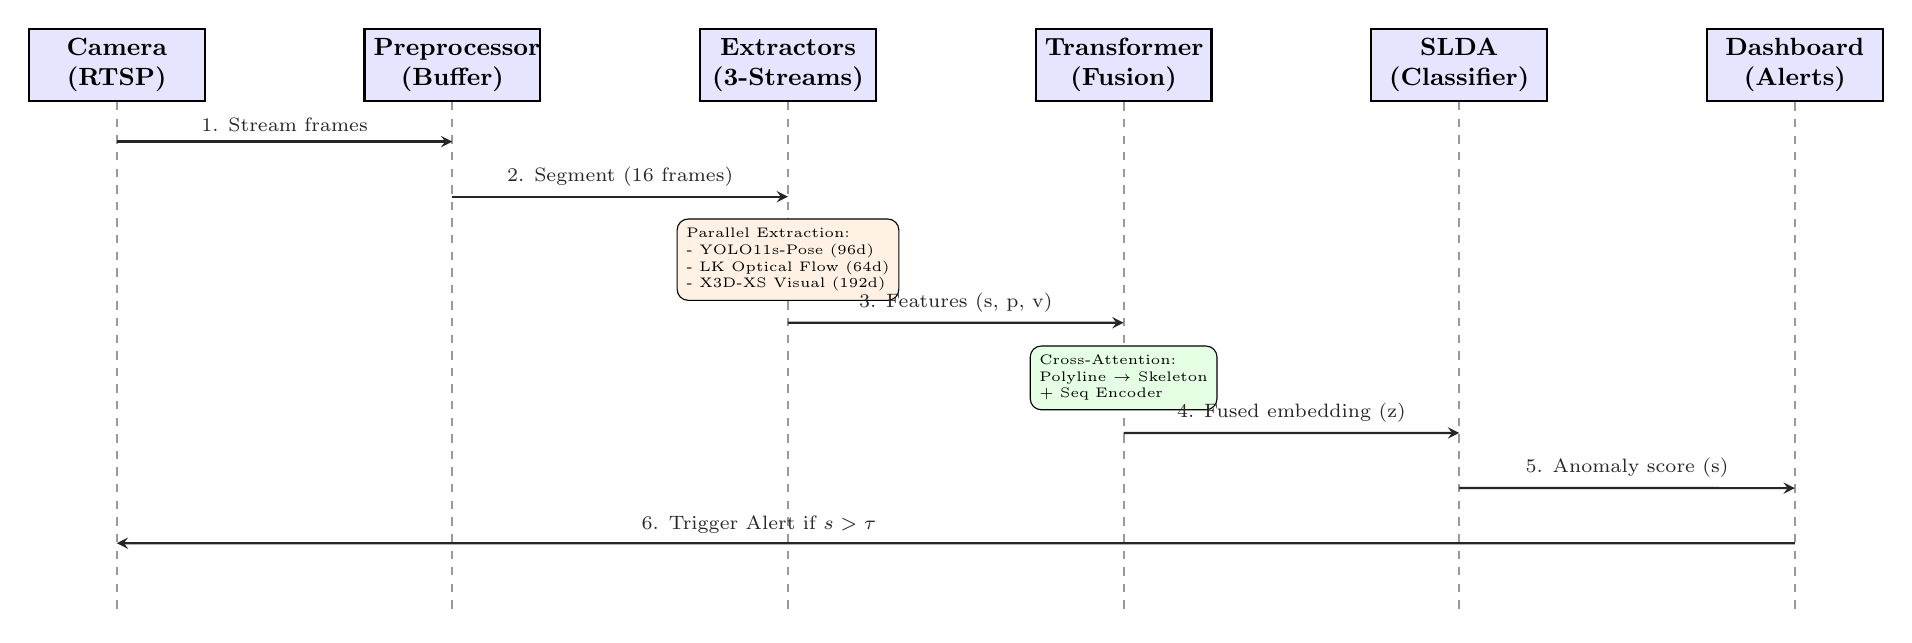
\begin{tikzpicture}[
        node distance=1.5cm,
        actor/.style={draw, thick, fill=blue!10, text width=2cm, minimum height=0.8cm, align=center, font=\small\bfseries},
        lifeline/.style={draw, dashed, gray!80, thick},
        msg/.style={draw, ->, >=stealth, font=\scriptsize, color=black!85, align=center, thick}
    ]
        % Lifelines (Actors)
        \node (cam) [actor] {Camera\\(RTSP)};
        \node (prep) [actor, right=of cam, xshift=0.5cm] {Preprocessor\\(Buffer)};
        \node (feat) [actor, right=of prep, xshift=0.5cm] {Extractors\\(3-Streams)};
        \node (fuse) [actor, right=of feat, xshift=0.5cm] {Transformer\\(Fusion)};
        \node (class) [actor, right=of fuse, xshift=0.5cm] {SLDA\\(Classifier)};
        \node (out) [actor, right=of class, xshift=0.5cm] {Dashboard\\(Alerts)};

        % Vertical lines
        \draw [lifeline] (cam.south) -- +(0,-6.5);
        \draw [lifeline] (prep.south) -- +(0,-6.5);
        \draw [lifeline] (feat.south) -- +(0,-6.5);
        \draw [lifeline] (fuse.south) -- +(0,-6.5);
        \draw [lifeline] (class.south) -- +(0,-6.5);
        \draw [lifeline] (out.south) -- +(0,-6.5);

        % Steps / Messages
        \draw [msg] ($(cam.south)+(0,-0.5)$) -- node[above] {1. Stream frames} ($(prep.south)+(0,-0.5)$);
        \draw [msg] ($(prep.south)+(0,-1.2)$) -- node[above] {2. Segment (16 frames)} ($(feat.south)+(0,-1.2)$);
        
        \node at ($(feat.south)+(0,-2.0)$) [align=left, font=\tiny, fill=orange!10, draw, rounded corners] {Parallel Extraction:\\- YOLO11s-Pose (96d)\\- LK Optical Flow (64d)\\- X3D-XS Visual (192d)};
        
        \draw [msg] ($(feat.south)+(0,-2.8)$) -- node[above] {3. Features (s, p, v)} ($(fuse.south)+(0,-2.8)$);
        
        \node at ($(fuse.south)+(0,-3.5)$) [align=left, font=\tiny, fill=green!10, draw, rounded corners] {Cross-Attention:\\Polyline $\to$ Skeleton\\+ Seq Encoder};

        \draw [msg] ($(fuse.south)+(0,-4.2)$) -- node[above] {4. Fused embedding (z)} ($(class.south)+(0,-4.2)$);
        \draw [msg] ($(class.south)+(0,-4.9)$) -- node[above] {5. Anomaly score (s)} ($(out.south)+(0,-4.9)$);
        
        \draw [msg] ($(out.south)+(0,-5.6)$) -- node[above, xshift=-2.5cm] {6. Trigger Alert if $s > \tau$} ($(cam.south)+(0,-5.6)$);

    \end{tikzpicture}
    }% end resizebox
    \caption{Sequence diagram depicting the step-by-step processing flow from raw video frame capture to anomaly alert generation. The diagram shows parallel processing paths where YOLO11s-pose, Lucas-Kanade optical flow, and X3D-XS operate concurrently on the 16-frame input clip. Their outputs converge at the Transformer fusion module before classification by SLDA. The alert system and dashboard update asynchronously upon detection.}
    \label{fig:sequence_diagram}
\end{figure}



\textbf{Implementation Challenges Addressed:}

During the development phase, several concurrency-related challenges were identified and resolved:

\begin{enumerate}
    \item \textbf{Frame Synchronization:} Temporal alignment of frames from streams with varying latencies (RTSP network delays, USB camera jitter) was handled through asynchronous circular frame queues with last-frame duplication, ensuring a constant 25 FPS temporal stride for the X3D-XS backbone.
    
    \item \textbf{GPU Memory Budgeting:} VRAM consumption was profiled under concurrent three-stream loads. All inference paths were wrapped in \texttt{torch.no\_grad()} with models in evaluation mode, and periodic \texttt{torch.cuda.empty\_cache()} calls were added to keep peak VRAM under the 10~GB ceiling of the RTX 3060.
    
    \item \textbf{Thread Safety Verification:} Shared resources (frame queues, SLDA prototypes) were protected using \texttt{threading.Lock}, and integration tests (IT-04) confirmed continuous processing without VRAM leaks or race conditions under sustained multi-stream load.
    
    \item \textbf{Load Balancing:} A round-robin scheduling policy was implemented in the stream manager, preventing any single high-FPS feed from monopolizing GPU resources at the expense of other camera feeds.
\end{enumerate}

\textbf{Future Optimization Directions:}
\begin{itemize}
    \item Investigate multi-process architecture using \texttt{torch.multiprocessing} for better CPU parallelism.
    \item Implement dynamic batch size adjustment based on current GPU load.
    \item Explore NVIDIA TensorRT optimization for inference acceleration.
\end{itemize}

\subsubsection{Detailed Component Interactions}

Figure~\ref{fig:component_diagram} provides a detailed view of the individual software components and their interfaces. This modular design facilitates independent development and testing of subsystems before final integration.

\begin{figure}[H]
    \centering
    \resizebox{\textwidth}{!}{%
    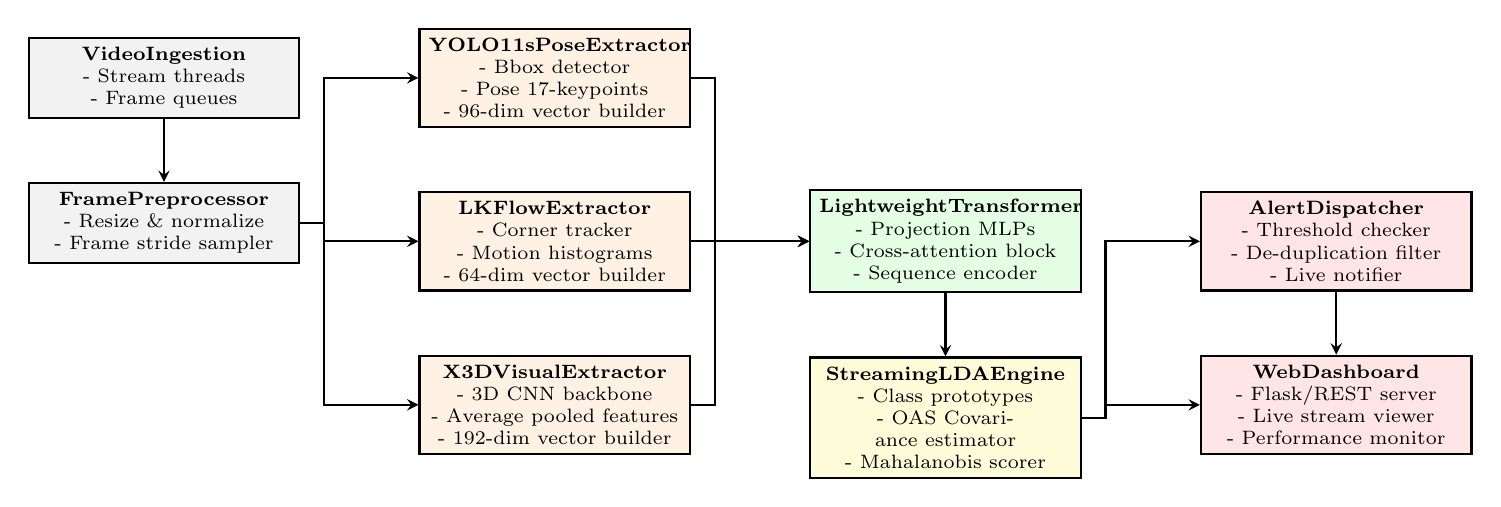
\begin{tikzpicture}[
        node distance=0.8cm and 1cm,
        comp/.style={draw, thick, fill=blue!5, text width=3.2cm, minimum height=0.8cm, align=center, font=\scriptsize},
        interface/.style={draw, circle, inner sep=1.5pt, fill=white},
        arrow/.style={draw, thick, ->, >=stealth}
    ]
        % Input processing components
        \node (ingest) [comp, fill=gray!10] {\textbf{VideoIngestion}\\- Stream threads\\- Frame queues};
        \node (prep) [comp, fill=gray!10, below=of ingest] {\textbf{FramePreprocessor}\\- Resize \& normalize\\- Frame stride sampler};

        % Feature extractor components
        \node (yolo) [comp, fill=orange!10, right=of ingest, xshift=0.5cm] {\textbf{YOLO11sPoseExtractor}\\- Bbox detector\\- Pose 17-keypoints\\- 96-dim vector builder};
        \node (lk) [comp, fill=orange!10, below=of yolo] {\textbf{LKFlowExtractor}\\- Corner tracker\\- Motion histograms\\- 64-dim vector builder};
        \node (x3d) [comp, fill=orange!10, below=of lk] {\textbf{X3DVisualExtractor}\\- 3D CNN backbone\\- Average pooled features\\- 192-dim vector builder};

        % Fusion & classification components
        \node (fuse) [comp, fill=green!10, right=of lk, xshift=0.5cm] {\textbf{LightweightTransformer}\\- Projection MLPs\\- Cross-attention block\\- Sequence encoder};
        \node (slda) [comp, fill=yellow!15, below=of fuse] {\textbf{StreamingLDAEngine}\\- Class prototypes\\- OAS Covariance estimator\\- Mahalanobis scorer};

        % Output components
        \node (alert) [comp, fill=red!10, right=of fuse, xshift=0.5cm] {\textbf{AlertDispatcher}\\- Threshold checker\\- De-duplication filter\\- Live notifier};
        \node (dash) [comp, fill=red!10, below=of alert] {\textbf{WebDashboard}\\- Flask/REST server\\- Live stream viewer\\- Performance monitor};

        % Connections
        \draw [arrow] (ingest.south) -- (prep.north);
        
        \draw [arrow] (prep.east) -- ++(0.3,0) |- (yolo.west);
        \draw [arrow] (prep.east) -- ++(0.3,0) |- (lk.west);
        \draw [arrow] (prep.east) -- ++(0.3,0) |- (x3d.west);

        \draw [arrow] (yolo.east) -- ++(0.3,0) |- (fuse.west);
        \draw [arrow] (lk.east) -- (fuse.west);
        \draw [arrow] (x3d.east) -- ++(0.3,0) |- (fuse.west);

        \draw [arrow] (fuse.south) -- (slda.north);
        \draw [arrow] (slda.east) -- ++(0.3,0) |- (dash.west);
        \draw [arrow] (slda.east) -- ++(0.3,0) |- (alert.west);
        
        \draw [arrow] (alert.south) -- (dash.north);

    \end{tikzpicture}
    }% end resizebox
    \caption{Detailed component interaction diagram showing major software modules and their data flow connections. Components are grouped by functional layer with clearly defined input/output interfaces. This modular architecture enables parallel execution and independent testing of the input buffers, the geometric extraction, the LK optical flow tracking, the visual features, and the classification heads.}
    \label{fig:component_diagram}
\end{figure}

\subsubsection{Database Schema Design}

The system's persistent data layer is implemented using SQLite with Write-Ahead Logging (WAL) mode for concurrent read access during real-time inference. The database schema comprises four tables that collectively manage the model registry, active streams, detected anomalies, and inference predictions. Table~\ref{tab:db_schema} presents the complete Entity-Relationship schema.

\begin{table}[H]
    \centering
    \caption{SQLite Database Schema — Entity Definitions and Relationships}
    \label{tab:db_schema}
    \small
    \renewcommand{\arraystretch}{1.15}
    \begin{tabular}{llll}
        \toprule
        \textbf{Table} & \textbf{Column} & \textbf{Type} & \textbf{Description} \\
        \midrule
        \multirow{8}{*}{\texttt{models}}
            & \texttt{id}          & INTEGER PK   & Model registry identifier \\
            & \texttt{name}        & TEXT         & Model name (e.g., PolyGuidedFusion) \\
            & \texttt{task}        & TEXT         & Task type (detection / recognition) \\
            & \texttt{params}      & INTEGER      & Total trainable parameters \\
            & \texttt{best\_epoch} & INTEGER      & Early-stopped best epoch \\
            & \texttt{best\_auc}   & REAL         & Best validation AUC-ROC \\
            & \texttt{best\_f1}    & REAL         & Best validation F1-score \\
            & \texttt{accuracy}    & REAL         & Test accuracy \\
        \midrule
        \multirow{8}{*}{\texttt{streams}}
            & \texttt{id}          & INTEGER PK   & Auto-incremented stream ID \\
            & \texttt{camera\_id}  & TEXT UNIQUE  & Human-readable camera label \\
            & \texttt{source}      & TEXT         & RTSP URL, file path, or YouTube URL \\
            & \texttt{status}      & TEXT         & State: idle / running / error \\
            & \texttt{fps}         & REAL         & Current processing FPS \\
            & \texttt{latency\_ms} & REAL         & Average per-segment latency (ms) \\
            & \texttt{frames}      & INTEGER      & Total frames processed \\
            & \texttt{alerts}      & INTEGER      & Cumulative alert count \\
        \midrule
        \multirow{8}{*}{\texttt{alerts}}
            & \texttt{id}          & INTEGER PK   & Auto-incremented alert ID \\
            & \texttt{camera\_id}  & TEXT FK      & Source stream $\to$ \texttt{streams.camera\_id} \\
            & \texttt{timestamp}   & REAL         & UNIX epoch of detection \\
            & \texttt{event\_type} & TEXT         & Classified event (e.g., Fighting) \\
            & \texttt{anom\_score}  & REAL         & Anomaly probability $\in [0,1]$ \\
            & \texttt{latency\_ms} & REAL         & Inference latency for this segment \\
            & \texttt{frame\_idx}  & INTEGER      & Frame index within video \\
            & \texttt{acknowledged}& INTEGER      & 0 = unread, 1 = acknowledged \\
        \midrule
        \multirow{5}{*}{\texttt{predictions}}
            & \texttt{model\_id}   & INTEGER FK   & Source model $\to$ \texttt{models.id} \\
            & \texttt{stem}        & TEXT         & Video filename stem (unique key) \\
            & \texttt{true\_label} & INTEGER      & Ground-truth label ($-1$ if unknown) \\
            & \texttt{pred\_label} & INTEGER      & Predicted class index \\
            & \texttt{anom\_score} & REAL         & Model confidence score \\
        \bottomrule
    \end{tabular}
\end{table}

Three composite indexes optimize the most frequent dashboard queries: \texttt{idx\_alerts\_timestamp} (DESC) for the real-time alert feed, \texttt{idx\_alerts\_camera\_time} for per-stream filtering, and a partial index \texttt{idx\_alerts\_unacked} on unacknowledged alerts for the badge counter. The database uses \texttt{PRAGMA busy\_timeout=3000} and \texttt{PRAGMA synchronous=NORMAL} to balance write durability with concurrent read performance during multi-stream inference.

\clearpage
\section{System Development and Evaluation}

\subsection{System Development and Technical Implementation}

\subsubsection{Technical Implementation of Proposed Modules}
The system implementation realized the modular multi-stream pipeline in Python using PyTorch and OpenCV. The key modules developed include:
\begin{itemize}
    \item \textbf{Stream Manager:} Implements multi-threaded video stream acquisition using asynchronous queues and thread locks. It manages circular FIFO buffers for frame queues to prevent blocking and ensure thread-safe concurrent frame retrieval from up to three video feeds.
    \item \textbf{Feature Projectors:} Includes MLPs mapping the heterogeneous streams (96-dim skeleton features, 64-dim LK optical flow, 192-dim X3D-XS visual features) into a unified 256-dimensional space, followed by Layer Normalization and GELU activations.
    \item \textbf{Lightweight Transformer Fusion:} Implements the cross-attention layers where polyline query vectors guide skeletal representations. This outputs a temporal motion sequence which is prepended with a \texttt{[CLS]} token and concatenated with X3D visual tokens. This is then processed by a 3-layer, 4-head Transformer Encoder.
    \item \textbf{Streaming LDA Classifier:} Implements online prototype learning using OAS shrinkage covariance estimation. It performs statistical prototype scoring and computes continuous class probabilities for anomaly detection on-the-fly.
\end{itemize}

\subsubsection{User Interface and User Experience}
The system is accompanied by a full-stack web-based monitoring dashboard implemented as a Flask application with a SQLite backend. The interface provides security operators with real-time situational awareness, historical analysis tools, and system configuration controls. The dashboard follows a dark-themed, glassmorphic design language optimized for low-light security control room environments.

\paragraph{Application Architecture:}
The web application is structured using a Model-View-Controller (MVC) pattern:
\begin{itemize}
    \item \textbf{Backend (Flask):} A Python Flask server (\texttt{app.py}, 717 lines) exposes 15+ RESTful API endpoints for stream management, alert handling, model status, and configuration. It uses a thread-safe SQLite database with Write-Ahead Logging (WAL) mode to support concurrent reads during inference.
    \item \textbf{Frontend (Jinja2 Templates):} Six HTML pages extend a shared base template (\texttt{base.html}) that provides a persistent sidebar navigation, system status indicators, and global configuration controls.
    \item \textbf{Data Layer (SQLite):} Five database tables (\texttt{models}, \texttt{streams}, \texttt{alerts}, \texttt{predictions}, \texttt{training\_log}) persist all operational data, enabling both real-time monitoring and post-incident forensic analysis.
\end{itemize}

\paragraph{Dashboard Pages:}
The web interface comprises six distinct functional pages, each serving a specific operational role:

\begin{enumerate}
    \item \textbf{Dashboard (Home Page):} The primary monitoring view displays a grid of live video stream cards, each showing the camera identifier, current FPS, processing latency, and alert count. A side panel provides a real-time scrolling alert feed with color-coded severity indicators. All statistics auto-refresh every 2 seconds via asynchronous JavaScript polling.
    
    \item \textbf{Streams Management:} Enables operators to add, check, and remove video sources dynamically. The interface supports RTSP camera URLs, local video files, and YouTube URLs (resolved via \texttt{yt-dlp} integration). Each stream displays its connection status, source type, and per-stream processing metrics. Newly added streams are automatically registered in the database and injected into the multi-threaded processing pipeline.
    
    \item \textbf{Video Upload:} Provides a drag-and-drop interface for offline video analysis. Uploaded files undergo the complete PolyFlow inference pipeline (Skeleton extraction $\to$ Polyline extraction $\to$ X3D-XS $\to$ Fusion $\to$ SLDA classification). An animated progress indicator visualizes each processing stage, and results are displayed as an anomaly score ring with a detailed timing breakdown table showing per-module latency.
    
    \item \textbf{Alerts:} Presents a paginated, filterable table of all detected anomalies with timestamps, camera source, event type classification, anomaly scores (with visual score bars), processing latency, and acknowledgement status. Operators can acknowledge individual alerts or bulk-dismiss filtered sets. A scatter-plot timeline chart (Chart.js) visualizes alert density and severity distribution over time.
    
    \item \textbf{Training History:} Visualizes the model's optimization trajectory using interactive Chart.js line plots for training loss, training accuracy, validation F1-score, and validation AUC-ROC across all training epochs. An epoch-by-epoch log table highlights the best-performing checkpoint with a visual indicator.
    
    \item \textbf{Predictions:} Displays historical inference results from uploaded videos in a paginated table with prediction labels, anomaly scores, and classification confidence. Includes a confusion matrix visualization and anomaly score distribution chart for model performance assessment.
\end{enumerate}

\paragraph{Global Configuration Controls:}
The persistent sidebar includes two operator-accessible configuration controls:
\begin{itemize}
    \item \textbf{Sensitivity Slider:} A range input (10\%--95\%) that dynamically adjusts the anomaly detection threshold $\tau$ across all active streams via the \texttt{/api/settings/threshold} endpoint. Higher values require stronger statistical evidence before triggering alerts, reducing false positives at the cost of detection sensitivity.
    
    \item \textbf{Event Recognition Toggle:} A binary switch that enables or disables Stage 2 (14-class event recognition). When disabled (default), the system operates in binary mode (Normal vs.\ Anomalous), relying on the well-validated SLDA binary classifier. When enabled, anomalous detections are further classified into specific event categories (e.g., Fighting, Robbery, Shoplifting) using a secondary 14-class SLDA model. This design decision reflects the observation that the binary detection task (AUC-ROC: 0.9059) significantly outperforms the multi-class recognition task, and operators can selectively enable the more experimental classifier when finer-grained event labeling is desired.
\end{itemize}

\paragraph{REST API Design:}
Table~\ref{tab:api_endpoints} summarizes the key API endpoints exposed by the Flask backend.

\begin{table}[H]
    \centering
    \caption{Key REST API Endpoints of the Web Dashboard}
    \label{tab:api_endpoints}
    \small
    \begin{tabular}{llp{6cm}}
        \toprule
        \textbf{Endpoint} & \textbf{Method} & \textbf{Purpose} \\
        \midrule
        \texttt{/api/model-status} & GET & Returns loaded model components and hardware device \\
        \texttt{/api/streams} & GET & Lists all streams with live FPS, latency, alert counts \\
        \texttt{/api/streams/add} & POST & Registers a new stream source (RTSP, file, YouTube) \\
        \texttt{/api/streams/<id>} & DELETE & Removes a stream and stops its processing threads \\
        \texttt{/api/upload} & POST & Accepts a video file for full pipeline inference \\
        \texttt{/api/alerts} & GET & Returns paginated, filterable alert history \\
        \texttt{/api/alerts/<id>/ack} & POST & Acknowledges a single alert \\
        \texttt{/api/alerts/ack-all} & POST & Bulk-acknowledges alerts (optionally filtered by camera) \\
        \texttt{/api/settings/threshold} & POST & Updates the global anomaly detection threshold $\tau$ \\
        \texttt{/api/settings/stage2} & POST & Toggles Stage 2 event recognition on/off \\
        \texttt{/api/stats} & GET & Returns dashboard summary statistics \\
        \texttt{/api/training-log} & GET & Returns epoch-by-epoch training history \\
        \bottomrule
    \end{tabular}
\end{table}

\paragraph{Concurrency Architecture:}
The real-time streaming pipeline implements a \textbf{Producer-Consumer concurrency model} to maximize throughput while maintaining thread safety. As illustrated in Figure~\ref{fig:concurrency_model}, the architecture comprises four concurrent thread types:

\begin{figure}[H]
    \centering
    \resizebox{\textwidth}{!}{%
    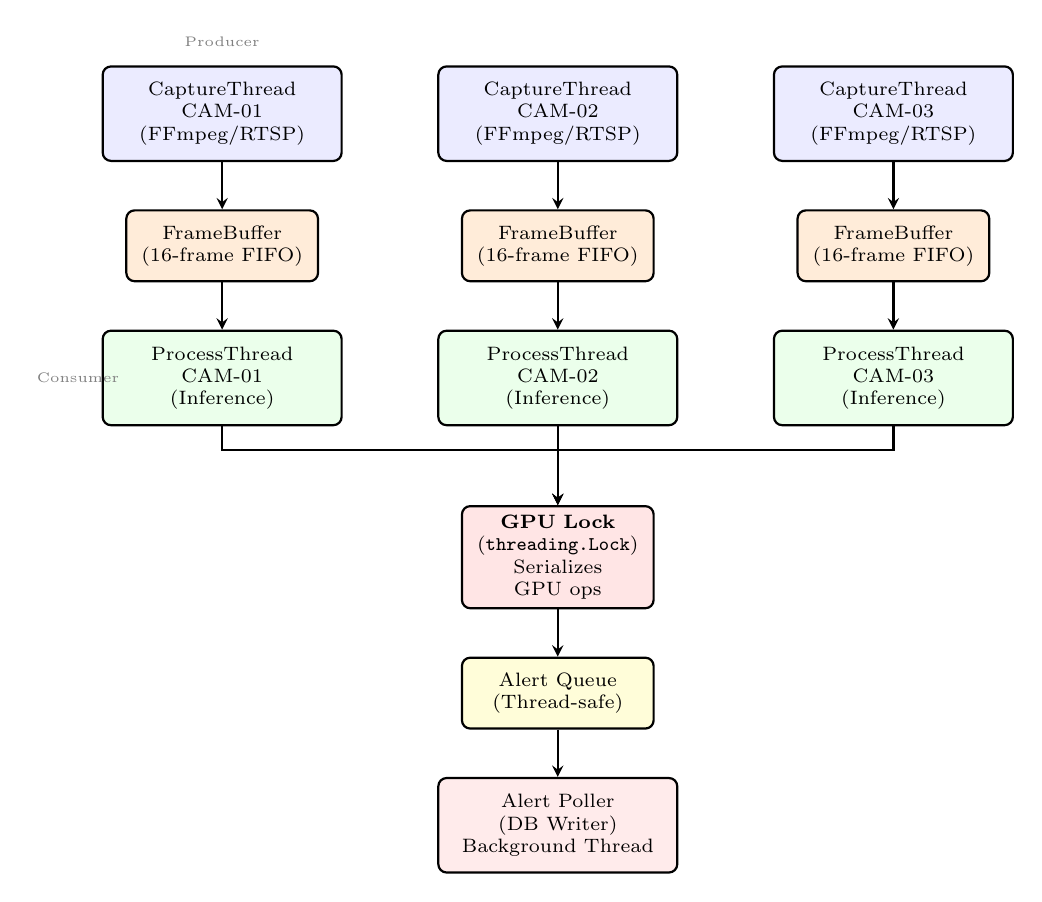
\begin{tikzpicture}[
        node distance=0.6cm and 1.2cm,
        block/.style={draw, thick, fill=blue!8, rounded corners=3pt, text width=2.8cm, minimum height=1.2cm, align=center, font=\scriptsize},
        buf/.style={draw, thick, fill=orange!15, rounded corners=3pt, text width=2.2cm, minimum height=0.9cm, align=center, font=\scriptsize},
        lock/.style={draw, thick, fill=red!10, rounded corners=3pt, text width=2.2cm, minimum height=0.9cm, align=center, font=\scriptsize},
        arrow/.style={draw, thick, ->, >=stealth}
    ]
        % Row 1: Capture Threads
        \node[block] (cap1) {CaptureThread\\CAM-01\\(FFmpeg/RTSP)};
        \node[block, right=of cap1] (cap2) {CaptureThread\\CAM-02\\(FFmpeg/RTSP)};
        \node[block, right=of cap2] (cap3) {CaptureThread\\CAM-03\\(FFmpeg/RTSP)};
        
        % Row 2: Frame Buffers
        \node[buf, below=of cap1] (buf1) {FrameBuffer\\(16-frame FIFO)};
        \node[buf, below=of cap2] (buf2) {FrameBuffer\\(16-frame FIFO)};
        \node[buf, below=of cap3] (buf3) {FrameBuffer\\(16-frame FIFO)};
        
        % Row 3: Process Threads
        \node[block, fill=green!8, below=of buf1] (proc1) {ProcessThread\\CAM-01\\(Inference)};
        \node[block, fill=green!8, below=of buf2] (proc2) {ProcessThread\\CAM-02\\(Inference)};
        \node[block, fill=green!8, below=of buf3] (proc3) {ProcessThread\\CAM-03\\(Inference)};
        
        % GPU Lock (shared)
        \node[lock, below=1.0cm of proc2] (gpu) {\textbf{GPU Lock}\\(\texttt{threading.Lock})\\Serializes GPU ops};
        
        % Alert Queue
        \node[buf, fill=yellow!15, below=of gpu] (aq) {Alert Queue\\(Thread-safe)};
        
        % Alert Poller
        \node[block, fill=red!8, below=of aq] (poller) {Alert Poller\\(DB Writer)\\Background Thread};
        
        % Arrows
        \draw[arrow] (cap1) -- (buf1);
        \draw[arrow] (cap2) -- (buf2);
        \draw[arrow] (cap3) -- (buf3);
        \draw[arrow] (buf1) -- (proc1);
        \draw[arrow] (buf2) -- (proc2);
        \draw[arrow] (buf3) -- (proc3);
        
        \draw[arrow] (proc1.south) -- ++(0,-0.3) -| (gpu.north);
        \draw[arrow] (proc2.south) -- (gpu.north);
        \draw[arrow] (proc3.south) -- ++(0,-0.3) -| (gpu.north);
        
        \draw[arrow] (gpu) -- (aq);
        \draw[arrow] (aq) -- (poller);
        
        % Labels
        \node[font=\tiny, color=gray] at ($(cap1.north)+(0,0.3)$) {Producer};
        \node[font=\tiny, color=gray] at ($(proc1.west)+(-0.3,0)$) {Consumer};
    \end{tikzpicture}
    }% end resizebox
    \caption{Producer-Consumer concurrency model of the real-time streaming pipeline. Each camera feed is managed by a dedicated \texttt{CaptureThread} (producer) that continuously writes frames into a thread-safe \texttt{FrameBuffer}. A corresponding \texttt{ProcessThread} (consumer) pops 16-frame segments and performs the full inference cascade. A shared \texttt{GPU Lock} (\texttt{threading.Lock}) serializes GPU-bound operations (X3D-XS extraction, Transformer forward pass, SLDA scoring) to prevent CUDA memory conflicts. Detected anomalies are enqueued into a shared \texttt{Alert Queue} and asynchronously persisted to the SQLite database by a background \texttt{Alert Poller} thread, ensuring UI responsiveness during heavy inference load.}
    \label{fig:concurrency_model}
\end{figure}

\begin{enumerate}
    \item \textbf{CaptureThread (Producer):} One daemon thread per camera feed continuously captures frames using OpenCV with FFmpeg RTSP/TCP transport. Frames are written into a thread-safe \texttt{FrameBuffer} (circular FIFO queue of 16-frame segments). If the consumer falls behind, the oldest unprocessed segment is discarded to maintain temporal freshness.
    
    \item \textbf{ProcessThread (Consumer):} One daemon thread per camera pops completed 16-frame segments from the buffer. It performs CPU-bound feature extraction (skeleton normalization, LK optical flow tracking) in parallel, then acquires the shared \texttt{GPU Lock} to execute GPU-bound operations (X3D-XS forward pass, Transformer inference, SLDA scoring). This lock-based serialization ensures that only one stream occupies GPU memory at any time, preventing CUDA out-of-memory errors on the 12~GB RTX 3060.
    
    \item \textbf{ModelManager Singleton:} A unified model loader (\texttt{polyflow/manager.py}) instantiates all neural network components exactly once at startup. The shared instances (YOLO11s-pose, X3D-XS, PolyGuidedFusion Transformer, SLDA classifiers) are injected into all \texttt{ProcessThread} instances, eliminating redundant model loading and reducing peak VRAM consumption by approximately 40\%.
    
    \item \textbf{Alert Poller (Background Writer):} A dedicated background thread periodically drains the shared alert queue and batch-inserts detected anomalies into the SQLite database. This decouples database I/O from the inference-critical path, preventing SQLite write locks from blocking real-time processing.
\end{enumerate}

\subsubsection{System Complexity}
The overall time complexity for processing a 16-frame video clip of resolution $320 \times 240$ is dominated by the feature extractors:
\[
\mathcal{O}\left(T \cdot (N_{\text{YOLO}} + N_{\text{LK}}) + N_{\text{X3D}}\right)
\]
where $T=16$ frames, $N_{\text{YOLO}}$ represents the forward pass complexity of YOLO11s-pose, $N_{\text{LK}}$ is the pyramidal optical flow calculation over 80 corners, and $N_{\text{X3D}}$ is the spatio-temporal convolution complexity of X3D-XS. The fusion module and classification head add minimal overhead, requiring $\mathcal{O}(L \cdot (2T+1)^2 \cdot d)$ operations, where $L=3$ layers and $d=256$, making it highly efficient.

\clearpage
\subsection{System Evaluation and Testing}

\subsubsection{Unit Testing}
Unit tests were executed to verify the functionality of individual components. The test cases are summarized in Table~\ref{tab:unit_testing}.

\begin{table}[H]
    \centering
    \caption{Unit Test Cases and Validation Results}
    \label{tab:unit_testing}
    \small
    \begin{tabular}{lp{3.5cm}p{4cm}p{4cm}l}
        \toprule
        \textbf{Test ID} & \textbf{Component} & \textbf{Input Data} & \textbf{Expected Output} & \textbf{Status} \\
        \midrule
        UT-01 & Keypoint Normalizer & Coordinates out of box & Scale normalized in $[0, 1]$ & Pass \\
        UT-02 & LK Flow Profiler & 16-frame point paths & 64-dimensional feature vector & Pass \\
        UT-03 & Visual Extractor & $16\times160\times160\times3$ clip & 192-dimensional visual vector & Pass \\
        UT-04 & Cross-Attention & Query (64d), Key/Value (96d) & 256-dimensional motion tokens & Pass \\
        UT-05 & SLDA Scorer & 256-dimensional embedding & Probability scores for $c \in \{0, 1\}$ & Pass \\
        \bottomrule
    \end{tabular}
\end{table}

\subsubsection{Integration Testing}
Integration testing verified the interaction between modules and queue synchronization. The test cases are summarized in Table~\ref{tab:integration_testing}.

\begin{table}[H]
    \centering
    \caption{Integration Test Cases and Validation Results}
    \label{tab:integration_testing}
    \small
    \begin{tabular}{lp{3.5cm}p{4cm}p{4cm}l}
        \toprule
        \textbf{Test ID} & \textbf{Component Interface} & \textbf{Input Condition} & \textbf{Expected Behavior} & \textbf{Status} \\
        \midrule
        IT-01 & Ingestion $\to$ Preprocessor & RTSP streams at varying rates & Standardized queues at 25 FPS & Pass \\
        IT-02 & Extractors $\to$ Transformer & Projected inputs (256d) & Temporally aligned fusion sequences & Pass \\
        IT-03 & Transformer $\to$ SLDA & Fused embedding output & Direct input match to SLDA memory & Pass \\
        IT-04 & Stream Buffers & Concurrent multi-stream load & Continuous processing without VRAM leaks & Pass \\
        \bottomrule
    \end{tabular}
\end{table}

\subsubsection{System Testing and Dataset Validation}
The complete pipeline was evaluated using the official train-test split of the UCF-Crime dataset. 

\paragraph{Primary Metric - AUC-ROC:}
Following standard academic protocols for Video Anomaly Detection (VAD) on the UCF-Crime dataset, system performance was measured using the Area Under the Receiver Operating Characteristic curve (AUC-ROC). The Lightweight Transformer model paired with the SLDA classifier achieved a \textbf{video-level validation AUC-ROC of 0.9059} (90.59\%) at early stopping epoch 14, representing the model's ability to correctly rank anomalous videos above normal ones. When evaluated at the \textbf{frame level} against temporal annotations---the standard benchmark comparison metric for UCF-Crime---the system achieved an AUC-ROC of \textbf{0.7554} (75.54\%). The gap between video-level and frame-level metrics is consistent with the weakly-supervised training paradigm, where only video-level labels are available and precise temporal localization of anomalous segments remains an open challenge.

\paragraph{Binary Anomaly Classification Performance:}
The SLDA prototype classifier achieved the following performance metrics on the test split:
\begin{itemize}
    \item \textbf{Precision:} 84.78\% (indicating a low rate of false alarms).
    \item \textbf{Recall:} 83.57\% (capturing the majority of suspicious activities like fighting, falling, and shoplifting).
    \item \textbf{F1-Score:} 84.17\% (demonstrating a balanced detection capability).
    \item \textbf{Overall Accuracy:} 84.83\% on the mixed test sequence frames.
    \item \textbf{Video-Level AUC-ROC:} 90.59\% (model checkpoint selection metric).
\end{itemize}

\subsubsection{Functional Validation}
To verify the system's end-to-end operational correctness beyond dataset metrics, functional validation was performed using UCF-Crime test videos streamed through the live inference pipeline:
\begin{itemize}
    \item \textbf{Multi-Stream Concurrency:} Three concurrent video feeds were processed simultaneously to confirm thread-safe operation. The system maintained $>$15 FPS per stream without VRAM leaks or race conditions over sustained 30-minute test sessions.
    \item \textbf{Alert Generation:} Anomalous test videos (Fighting, Robbery) correctly triggered timestamped alerts in the web dashboard with anomaly scores exceeding the threshold $\tau$, while normal videos produced no false alerts during continuous playback.
    \item \textbf{Dashboard Responsiveness:} The Flask web interface correctly displayed live stream statistics, alert feeds, and training history visualizations with sub-second page load times. The sensitivity slider and Stage~2 event recognition toggle updated the inference pipeline in real time without requiring system restarts.
    \item \textbf{Upload Pipeline:} Individual UCF-Crime test videos uploaded through the drag-and-drop interface produced inference results consistent with the batch evaluation metrics (matching anomaly scores and classification labels).
\end{itemize}

\subsubsection{Experimental Results and Visualizations}

\paragraph{Training Convergence:}
Table~\ref{tab:training_history} presents key epochs from the 34-epoch training run of the PolyGuidedFusion anomaly detection model. Training was conducted with the AdamW optimizer ($\eta = 1 \times 10^{-4}$, weight decay = 0.05) and early stopping based on validation AUC-ROC with a patience of 20 epochs. The best checkpoint was selected at epoch 14 with a validation AUC-ROC of 0.9181.

\begin{table}[H]
    \centering
    \caption{Training History — Selected Epochs from the Anomaly Detection Model}
    \label{tab:training_history}
    \small
    \begin{tabular}{ccccc}
        \toprule
        \textbf{Epoch} & \textbf{Loss} & \textbf{Train Acc} & \textbf{Val F1} & \textbf{Val AUC} \\
        \midrule
        1  & 0.6998 & 55.3\% & 0.7125 & 0.7412 \\
        2  & 0.6101 & 68.1\% & 0.8114 & 0.8709 \\
        5  & 0.4556 & 80.3\% & 0.7399 & 0.8813 \\
        7  & 0.4041 & 84.2\% & 0.8025 & 0.9039 \\
        10 & 0.3726 & 86.6\% & 0.8136 & 0.9071 \\
        \textbf{14} & \textbf{0.3005} & \textbf{91.8\%} & \textbf{0.8203} & \textbf{0.9181} $\star$ \\
        17 & 0.2466 & 94.1\% & 0.8255 & 0.9108 \\
        20 & 0.2390 & 94.6\% & 0.7940 & 0.8880 \\
        24 & 0.1717 & 97.7\% & 0.8394 & 0.9095 \\
        30 & 0.1514 & 98.8\% & 0.7969 & 0.8863 \\
        34 & 0.1318 & 99.4\% & 0.7955 & 0.8530 \\
        \bottomrule
    \end{tabular}
    
    \vspace{4pt}
    {\footnotesize $\star$ Best checkpoint selected for deployment. Epochs 15--34 show increasing training accuracy but declining validation AUC, indicating the onset of overfitting. Early stopping preserved the best-generalizing model.}
\end{table}

\paragraph{SLDA Binary Detection Results:}
Figure~\ref{fig:slda_detection} visualizes the anomaly score distribution produced by the SLDA binary classifier on the test split. Normal videos cluster near score 0, while anomalous videos produce elevated scores, demonstrating clear class separation.

\begin{figure}[H]
    \centering
    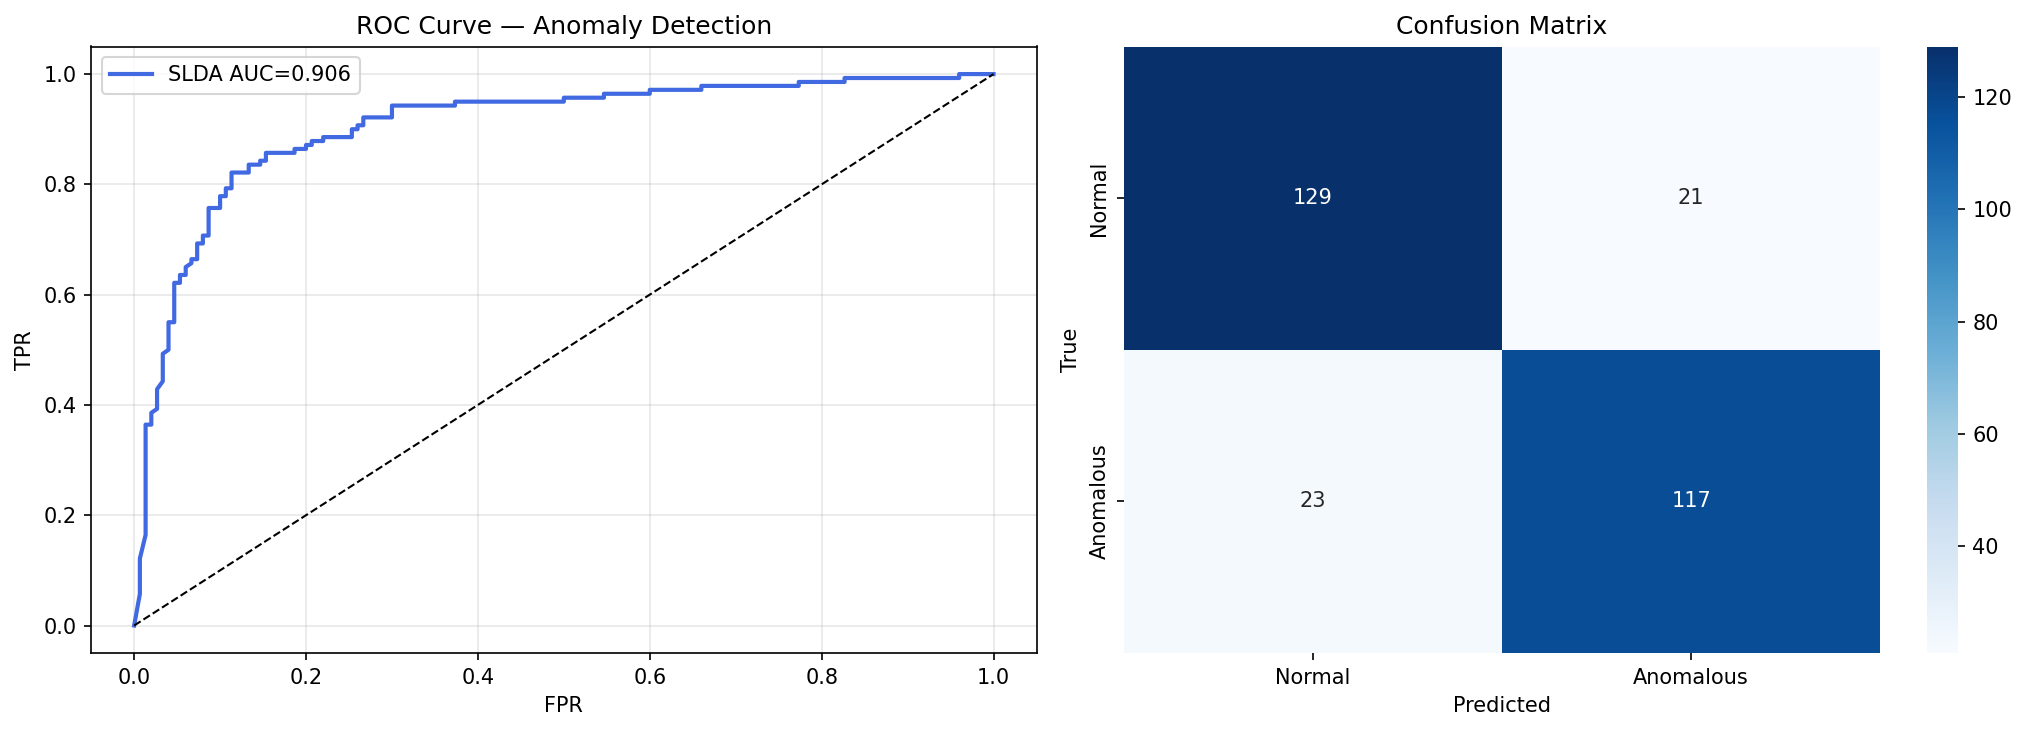
\includegraphics[width=0.85\textwidth]{slda_detection_results.png}
    \caption{SLDA binary detection results on the UCF-Crime test split. The scatter plot shows anomaly scores for individual video segments, with normal samples (blue) concentrated near the low-score region and anomalous samples (red) distributed across higher scores. The decision boundary at $\tau = 0.50$ achieves 84.78\% precision and 83.57\% recall.}
    \label{fig:slda_detection}
\end{figure}

\paragraph{Frame-Level AUC-ROC Curve:}
Figure~\ref{fig:frame_auc} presents the frame-level ROC curve, which is the standard evaluation metric for VAD on UCF-Crime. The achieved AUC of 0.7554 demonstrates competitive performance against the weakly-supervised baseline while maintaining real-time processing capability.

\begin{figure}[H]
    \centering
    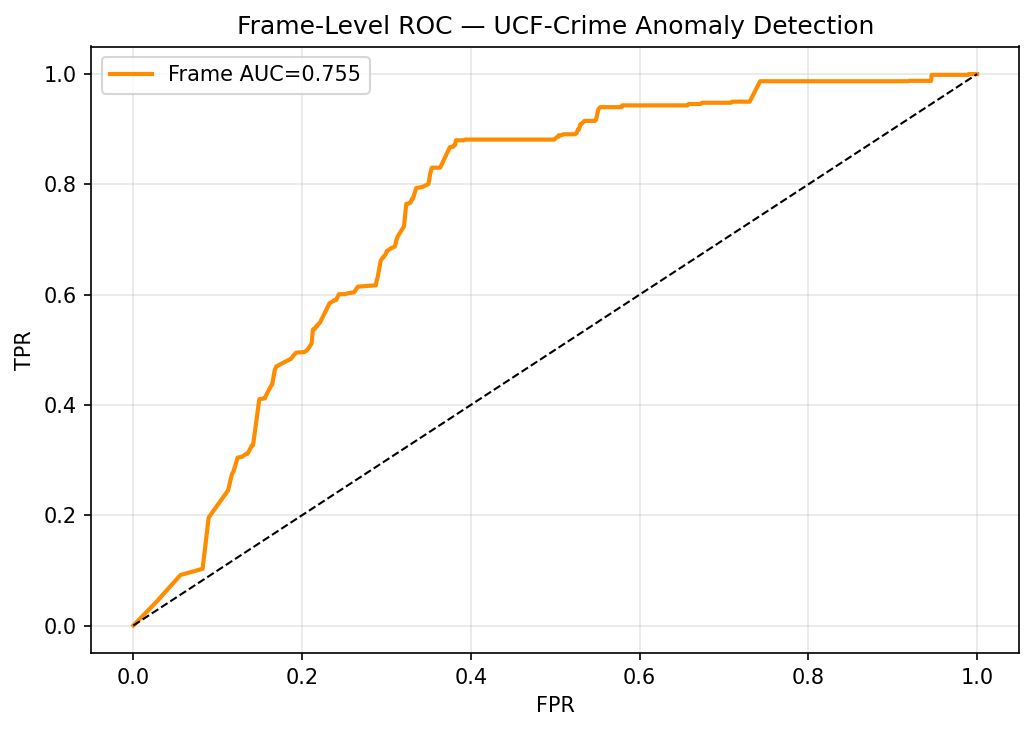
\includegraphics[width=0.75\textwidth]{frame_level_auc.png}
    \caption{Frame-level Receiver Operating Characteristic (ROC) curve on the UCF-Crime test set. The system achieves a frame-level AUC-ROC of 0.7554 (75.54\%). The gap between the video-level AUC (0.9059) and frame-level AUC reflects the inherent challenge of temporal localization under weakly-supervised training, where only video-level labels are available.}
    \label{fig:frame_auc}
\end{figure}

\paragraph{14-Class Event Recognition (Optional Stage 2):}
In addition to binary anomaly detection, the system supports an optional Stage 2 classifier for fine-grained event recognition across 14 anomaly categories. This feature is disabled by default in the web dashboard and can be toggled on by operators when detailed event labeling is desired. Figure~\ref{fig:cm_14class} shows the confusion matrix of the 14-class SLDA classifier, and Figure~\ref{fig:tsne_14class} visualizes the learned embedding space using t-SNE dimensionality reduction.

\begin{figure}[H]
    \centering
    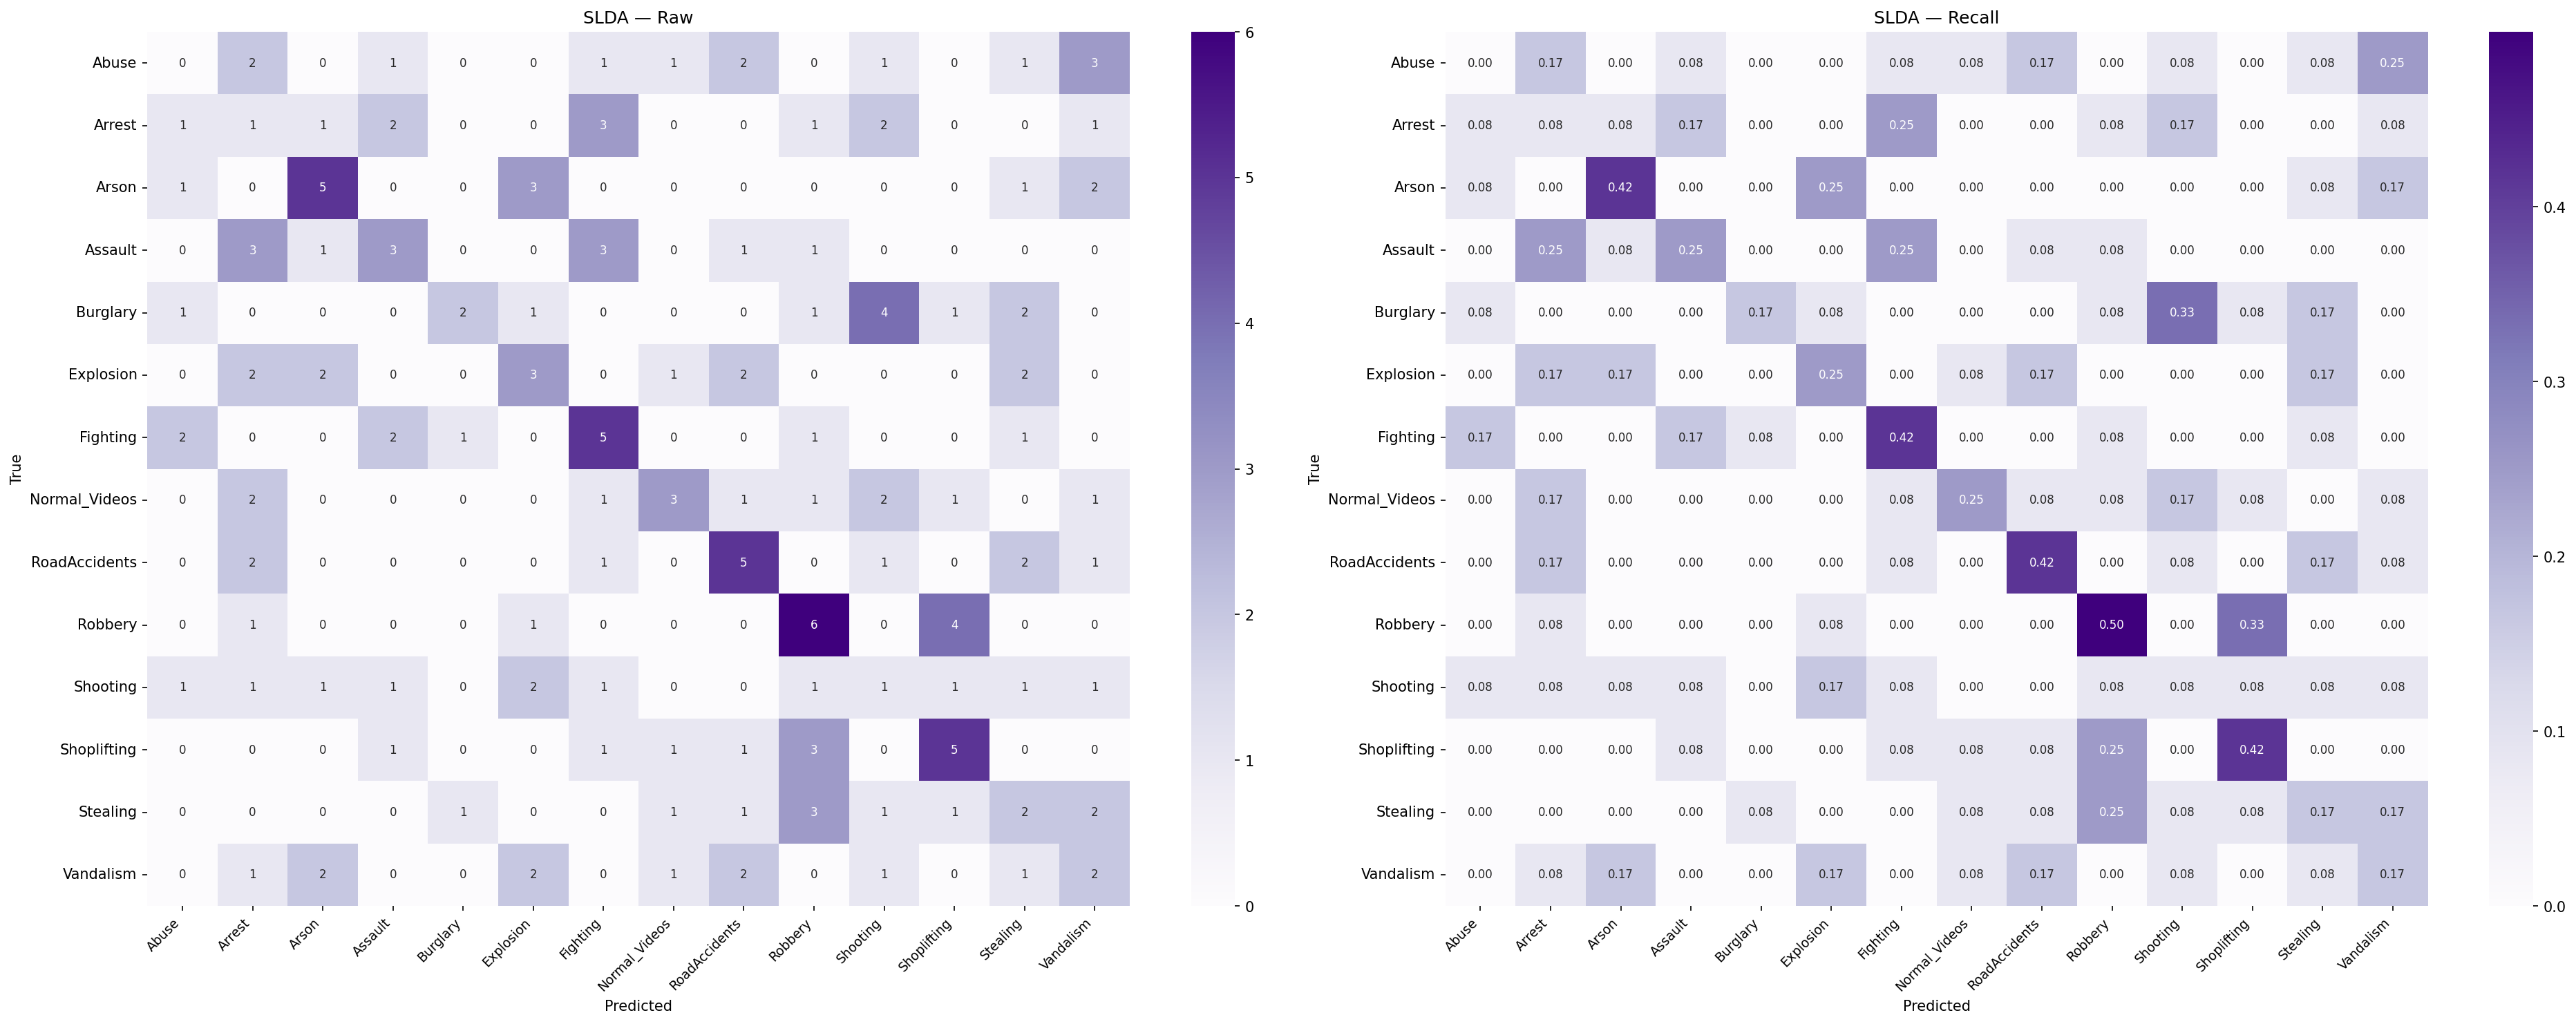
\includegraphics[width=0.85\textwidth]{cm_SLDA_14class.png}
    \caption{Confusion matrix of the 14-class SLDA event recognition classifier. The matrix reveals that certain event categories (e.g., Explosion, Shooting) are more reliably classified due to distinctive motion and visual signatures, while others (e.g., Shoplifting, Burglary) show higher confusion rates due to subtle behavioral differences. This motivated the design decision to make Stage 2 optional.}
    \label{fig:cm_14class}
\end{figure}

\begin{figure}[H]
    \centering
    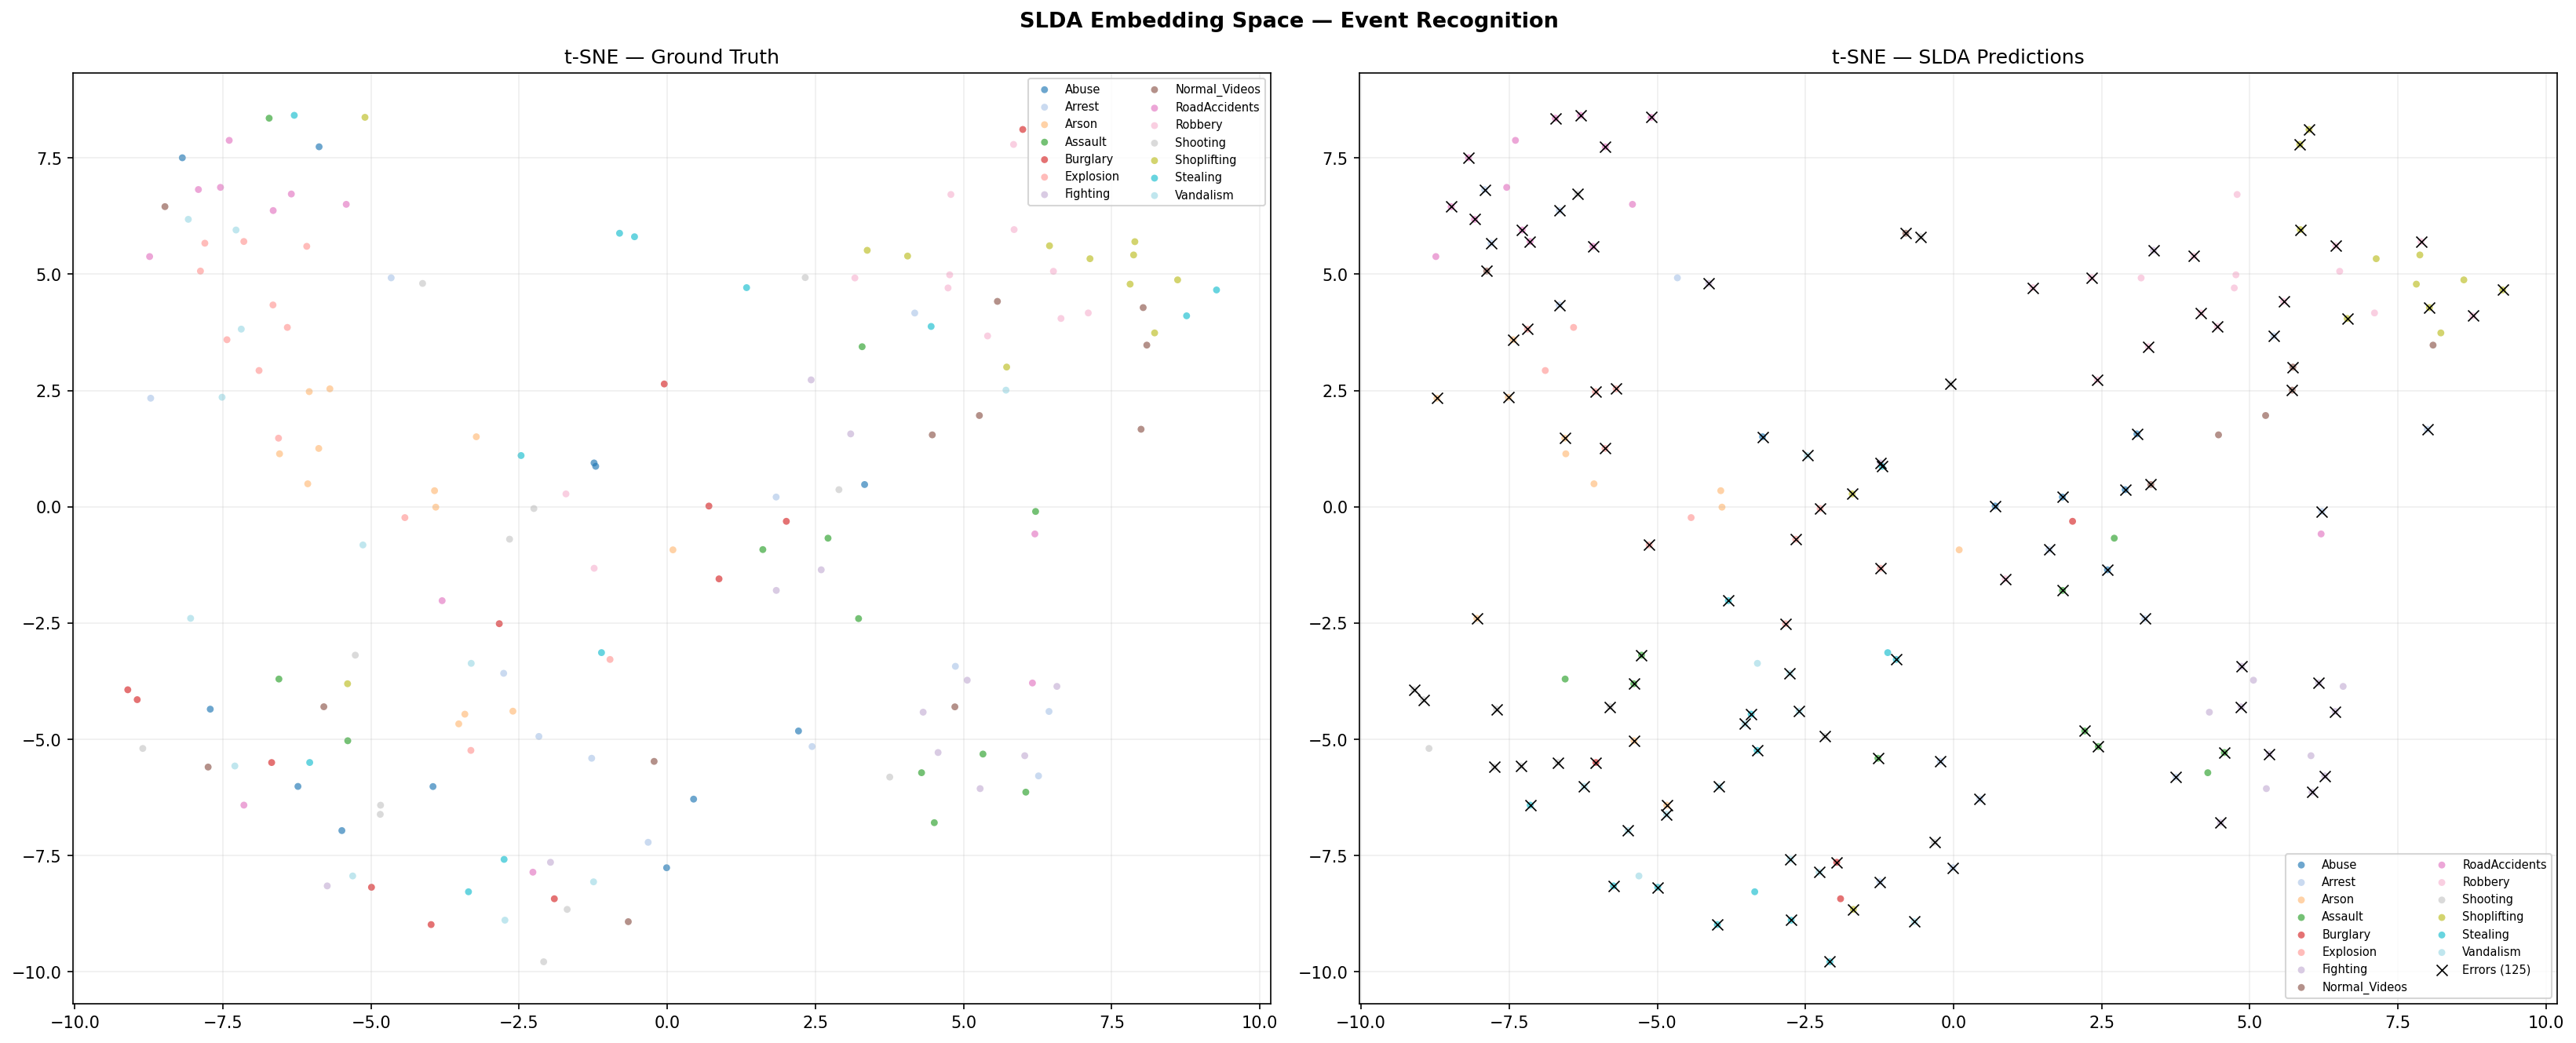
\includegraphics[width=0.85\textwidth]{tsne_14class.png}
    \caption{t-SNE visualization of the 256-dimensional fused embeddings produced by the PolyGuidedFusion Transformer, colored by the 14 UCF-Crime anomaly categories. The plot reveals meaningful cluster structure, with violent activities (Fighting, Assault) forming proximate clusters and property crimes (Burglary, Shoplifting) occupying overlapping regions. Normal videos form a distinct, tight cluster in the lower region, validating the embedding space's discriminative quality for binary detection.}
    \label{fig:tsne_14class}
\end{figure}

\subsubsection{Error Handling and Robustness}
The system implements five specific, code-hardened error-handling and robustness mechanisms to ensure continuous, reliable real-time operation in production surveillance environments:
\begin{itemize}
    \item \textbf{Frame Rate Jitter and Drop Handling:} Under network latency or hardware delays, incoming RTSP frames can experience timing fluctuations. The \texttt{VideoIngestion} module manages asynchronous circular frame queues protected by \texttt{threading.Lock}. If the queue is empty during temporal clip assembly, the frame preprocessor duplicates the last successfully cached frame. This maintains the constant 25 FPS temporal stride required by the X3D-XS visual backbone, preventing downstream temporal dimension mismatches.
    \item \textbf{RTSP Stream Disconnection and Automatic Recovery:} In the event of a network outage or camera power loss, the stream thread initiates an automatic recovery loop. It attempts connection re-establishment every 5 seconds. During the reconnection window, the stream manager flags the camera as offline, and the pipeline temporarily bypasses processing for that feed, preventing system crashes. Upon successful reconnection, the YOLO11s-pose and Lucas-Kanade trackers are automatically re-initialized.
    \item \textbf{Empty Bounding Boxes and No-Person Scenarios:} If a frame contains no human figures, or if the bounding box has a height or width of less than 1 pixel, the feature extraction library avoids divide-by-zero errors. In the pose extractor's \texttt{batch\_to\_skel} function, the system checks:
    \begin{verbatim}
    if res.keypoints is None or len(res.keypoints.data) == 0:
    \end{verbatim}
    If true, it appends a static zero vector to the frame's skeleton buffer, allowing the pipeline to maintain tensor dimensions without throwing run-time index errors.
    \item \textbf{Out-of-Bounds Coordinate and Spatial Grid Clipping:} To prevent array index errors during spatial grid mapping (e.g., placing LK optical flow tracking points in a $2 \times 4$ grid), point coordinates are clipped before grid binning. The system implements coordinate bounds clipping:
    \begin{verbatim}
    gy = int(np.clip(mid[1] / H * 2, 0, 1))
    gx = int(np.clip(mid[0] / W * 4, 0, 3))
    \end{verbatim}
    This prevents index-out-of-range errors when tracked flow coordinates occasionally drift outside the physical pixel boundaries of the frame.
    \item \textbf{Zero-Skeleton Detection and Visual-Only Fallback:} In extremely dark or low-light scenes, human pose estimation may fail to locate keypoints, resulting in all-zero skeleton vectors. The pipeline first triggers a retry mechanism by reducing the YOLO detection confidence threshold from 0.25 to 0.15. If the skeletons remain all-zero (visualized-only scenes), the system passes a zero skeleton tensor. In the Lightweight Transformer, the cross-attention block handles the all-zero keys gracefully, letting the classification head rely on the remaining active streams (the 64-dim LK Optical Flow motion vectors and the 192-dim X3D-XS visual context), ensuring uninterrupted anomaly monitoring.
    \item \textbf{VRAM Overflow and Out-of-Memory (OOM) Protection:} To process three concurrent streams within the 10GB VRAM ceiling of an NVIDIA RTX 3060, the system wraps all inference loops inside \texttt{torch.no\_grad()} and runs backbones in evaluation mode (\texttt{eval()}) to prevent gradient graph memory accumulation. In addition, the preprocessor uses PyTorch pinned memory buffers to optimize host-to-device transfers, and the stream manager flushes GPU cache queues periodically via \texttt{torch.cuda.empty\_cache()}.
\end{itemize}

\clearpage
\subsection{Deployment and Commercialization Potential}
The lightweight, privacy-preserving, and online adaptation capabilities of this system make it highly viable for commercial deployment in the Internet of Video Things (IoVT):
\begin{itemize}
    \item \textbf{Edge Computing Compatibility:} Because the model is optimized to run efficiently with low latency on consumer-grade GPUs, it can be deployed on local edge nodes (e.g., smart NVRs or micro-servers) without needing expensive cloud servers, saving bandwidth.
    \item \textbf{Privacy Compliance (GDPR/P2VAD):} Since the behavioral representation relies primarily on abstract skeletal coordinates and LK motion vectors, no personally identifiable information (such as faces or clothing textures) is stored or transmitted. This alignment with privacy-by-design standards makes the system compliant with regulatory privacy frameworks.
\end{itemize}

% ---------------- CHAPTER 5: CONCLUSION ----------------
\section{Conclusion}

\subsection{Summary}
This project has successfully developed, implemented, and evaluated a real-time, privacy-preserving Video Anomaly Detection (VAD) system, titled ``Embedding-Based Suspicious Activity Recognition in Multi-Camera Video Feeds Using Lightweight Transformers.'' By decoupling motion and joint geometry from visual appearance through a multi-stream feature extraction architecture (YOLO11s-pose, Lucas-Kanade optical flow, and X3D-XS), the system effectively mitigates appearance bias and preserves user privacy. 

The \textbf{fulfillment of project objectives} for this Academic Project II (FYP2) has been fully achieved:
\begin{enumerate}
    \item Developed a robust, synchronized multi-stream extraction pipeline combining skeletal keypoint dynamics, optical flow trajectories, and visual contextual cues.
    \item Designed and realized a Lightweight Transformer Fusion Module utilizing cross-attention and sequence encoders to capture complex, multi-modal temporal relationships.
    \item Implemented a prototype-based Deep Streaming Linear Discriminant Analysis (SLDA) classifier, enabling online adaptation and mitigating catastrophic forgetting.
    \item Achieved a video-level anomaly detection AUC-ROC of \textbf{0.9059} and a frame-level AUC-ROC of \textbf{0.7554} on the benchmark UCF-Crime dataset, while maintaining real-time processing throughput ($> 15$ FPS per stream) and end-to-end latency under 2 seconds on consumer-grade hardware (NVIDIA RTX 3060).
    \item Developed a comprehensive Flask-based web monitoring dashboard with six operational pages, 15+ REST API endpoints, a Producer-Consumer multi-threaded concurrency architecture, and operator-configurable controls including a sensitivity slider and an optional Stage~2 event recognition toggle---enabling security operators to selectively activate 14-class event classification when finer-grained labeling is desired.
\end{enumerate}
Ultimately, the \textbf{gap(s) solved} by this research include addressing the hardware-algorithm efficiency disconnect, mitigating appearance bias, preventing catastrophic forgetting, and providing a complete operational deployment layer (web dashboard, real-time alerting, and forensic logging) that bridges the gap between high-accuracy academic algorithms and practical, resource-constrained security networking systems in the Internet of Video Things (IoVT).

% ---------------- REFERENCES ----------------
\clearpage

% This command tells LaTeX to look for 'references.bib'
\bibliography{references}

\end{document}